\documentclass[conference]{IEEEtran}
\IEEEoverridecommandlockouts

\usepackage{cite}
\usepackage{amsmath}
\usepackage{amssymb}
\usepackage{amsfonts}
\usepackage{graphicx}
\usepackage{booktabs}
\usepackage{tikz}
\usetikzlibrary{positioning,arrows.meta,shapes.geometric,fit,backgrounds}
\usepackage{textcomp}
\usepackage{xcolor}
\usepackage{pifont}

\def\BibTeX{{\rm B\kern-.05em{\sc i\kern-.025em b}\kern-.08em
    T\kern-.1667em\lower.7ex\hbox{E}\kern-.125emX}}

\begin{document}

\title{Self-Supervised Continuous Domain Embeddings for Unified Multi-Sensor Satellite Image Translation}

% Double-blind build: pdflatex -jobname=main_anonymous "\def\ANON{}\documentclass[conference]{IEEEtran}
\IEEEoverridecommandlockouts

\usepackage{cite}
\usepackage{amsmath}
\usepackage{amssymb}
\usepackage{amsfonts}
\usepackage{graphicx}
\usepackage{booktabs}
\usepackage{tikz}
\usetikzlibrary{positioning,arrows.meta,shapes.geometric,fit,backgrounds}
\usepackage{textcomp}
\usepackage{xcolor}
\usepackage{pifont}

\def\BibTeX{{\rm B\kern-.05em{\sc i\kern-.025em b}\kern-.08em
    T\kern-.1667em\lower.7ex\hbox{E}\kern-.125emX}}

\begin{document}

\title{Self-Supervised Continuous Domain Embeddings for Unified Multi-Sensor Satellite Image Translation}

% Double-blind build: pdflatex -jobname=main_anonymous "\def\ANON{}\documentclass[conference]{IEEEtran}
\IEEEoverridecommandlockouts

\usepackage{cite}
\usepackage{amsmath}
\usepackage{amssymb}
\usepackage{amsfonts}
\usepackage{graphicx}
\usepackage{booktabs}
\usepackage{tikz}
\usetikzlibrary{positioning,arrows.meta,shapes.geometric,fit,backgrounds}
\usepackage{textcomp}
\usepackage{xcolor}
\usepackage{pifont}

\def\BibTeX{{\rm B\kern-.05em{\sc i\kern-.025em b}\kern-.08em
    T\kern-.1667em\lower.7ex\hbox{E}\kern-.125emX}}

\begin{document}

\title{Self-Supervised Continuous Domain Embeddings for Unified Multi-Sensor Satellite Image Translation}

% Double-blind build: pdflatex -jobname=main_anonymous "\def\ANON{}\documentclass[conference]{IEEEtran}
\IEEEoverridecommandlockouts

\usepackage{cite}
\usepackage{amsmath}
\usepackage{amssymb}
\usepackage{amsfonts}
\usepackage{graphicx}
\usepackage{booktabs}
\usepackage{tikz}
\usetikzlibrary{positioning,arrows.meta,shapes.geometric,fit,backgrounds}
\usepackage{textcomp}
\usepackage{xcolor}
\usepackage{pifont}

\def\BibTeX{{\rm B\kern-.05em{\sc i\kern-.025em b}\kern-.08em
    T\kern-.1667em\lower.7ex\hbox{E}\kern-.125emX}}

\begin{document}

\title{Self-Supervised Continuous Domain Embeddings for Unified Multi-Sensor Satellite Image Translation}

% Double-blind build: pdflatex -jobname=main_anonymous "\def\ANON{}\input{main.tex}"
% Camera-ready build (authors shown): pdflatex main.tex
\ifdefined\ANON
\author{
\IEEEauthorblockN{Anonymous Authors}
\IEEEauthorblockA{Anonymous Affiliation}
}
\else
\author{
\IEEEauthorblockN{Shivangi\textsuperscript{1}, Benedict Tephila M.\textsuperscript{2}, Naveen J.\textsuperscript{3}}
\IEEEauthorblockA{
Department of Computer Science and Engineering \\
CHRIST (Deemed to be University), Bangalore -- 560029, India \\
\textsuperscript{1}shivangi.a@mtech.christuniversity.in,
\textsuperscript{2}benedict.tephila@christuniversity.in,
\textsuperscript{3}naveen.j@christuniversity.in}
}
\fi

\maketitle

\begin{abstract}
The performance of deep learning models trained for the analysis of satellite images suffers when the same land-cover classes are captured by a different sensor, at a different season, or in a different region. Current domain-adaptation techniques typically require labeled target data, a fixed domain library, or both, but these are hard to obtain with evolving and expanding multi-sensor archives. Firstly, we present a continuous domain encoder that produces a label-free style embedding from unlabeled multi-sensor patches through the use of a contrastive (InfoNCE) pretext task, and secondly, we introduce a unified conditional generator that creates a style conditioned transformation of the content of the source patch into an arbitrary style of the target domain by learning a style embedding as a continuous latent space rather than a discrete class label. Both networks trained on 1,200 patches per sensor provided by PASTIS-HD (Sentinel-2, SPOT~6/7, Sentinel-1 SAR) and tested on 300 held-out patches per sensor from a region that is mostly different. The encoder successfully completes its pretext task, but recognises the sensor with only some success (65.8\% as opposed to 33.3\% chance). The generator maintains the scene structure and performs well on the pairs that contain SAR, but does not reproduce the radiometry of the target sensor: a constant image is closer to the actual target patch than a translation, and translated images end up as a source-independent color cast, when SAR is present in one of the pairs. This paper does not include generalization to unseen sensor pairs, nor does it include downstream accuracy.
\end{abstract}

\begin{IEEEkeywords}
domain adaptation, self-supervised learning, generative adversarial networks, contrastive learning, multi-sensor satellite imagery, image-to-image translation
\end{IEEEkeywords}

\section{Introduction}

Satellite remote sensing has now evolved from one single mission to a constellation of optical and radar satellites, seeing the Earth's surface together and in succession, such as Sentinel-2, Landsat, SPOT and a growing number of commercial very-high-resolution (VHR) and synthetic aperture radar (SAR) satellites. The use of deep learning models for land-cover classification, crop mapping and change detection has been increasingly placed on the ability to perform on this multi-sensor heterogeneous archive, as opposed to the single sensor they were trained on.

It is hard to achieve this cross-sensor requirement in practice. These include different radiometric calibration, spectral response, spatial resolution, and noise properties for each sensor, which vary from atmospheric haze and calibration drift in optical imagery to speckle noise and incidence-angle-dependent backscatter in SAR. Consequently, a model trained with the statistics from one sensor may exhibit a dramatic decrease in accuracy when applied to another sensor, even when the land-cover classes are the same. Modeling often requires the adaptation to a new domain with little or no target domain labeled data because of the high cost of acquiring and annotating imagery from all sensors of interest.

The current methods can be classified into two families. Satellite-specific methods, like multi-source standardization~\cite{tasar2020standardgan} normalize translation on a discrete domain identity that is manually assigned to each satellite and are claimed to have difficulty with unseen combinations of domains. However, self-supervised methods like SS(DA)$^2$~\cite{zhang2023ssdada} do not require labels or an explicit domain boundary and only translate between two satellites at a time, meaning that a new method must be developed for each new pair of satellites. In the general image-translation literature, StarGAN~\cite{choi2018stargan} and StarGAN~v2~\cite{choi2020starganv2} integrate a multitude of domains into a single generator, with StarGAN~v2 additionally using a continuous style code, and performing regular evaluations on natural images. Diffusion-based translators~\cite{vinholi2024multisensor,kieu2025universal} are more faithful but work on discrete domain sets, with higher inference cost.

The combination of label-free training, a continuous (discretely labeled is not the only option) representation of the domain and a single generator that can translate into an arbitrary target style is not yet explicitly provided in the literature for satellite images. It is the motivation for the present work to fill this gap.

The first two properties are addressed by further developing the pairwise approach of the SS(DA)$^2$ paradigm to a continuous, StarGAN~v2-style unified generator without the need for any domain-specific conditioning: A domain encoder produces a uniform embedding of the domain characteristics of each patch, and a single generator, modulated by the embedding through the use of AdaIN, maps a source patch to the domain of any target patch's embedding. These two components are designed, implemented, and evaluated using held-out data, which is not covered by this paper.

This paper makes the following contributions:
\begin{itemize}
\item A self-supervised contrastive domain encoder to generate label-free, continuous embeddings of sensor/style features from unlabeled multi-sensor patches.
A single AdaIN-modulated conditional generator conditioned on this embedding, instead of a discrete domain code, so no retraining per domain pair is required for the translation to an arbitrary target style.
An objective for six terms of training that maintains the geospatial content while changing the style of the content.
\item held out evaluation on real PASTIS-HD data that reports what works (label-free continuous embeddings, structure preserving, style conditioned translation) and what doesn't (moderate sensor information in the embedding, target radiometry not reproduced).
\end{itemize}

\section{Related Work}

\subsection{Domain Adaptation for Satellite Imagery}
StandardGAN~\cite{tasar2020standardgan} is used to standardize each source domain towards a common reference for semantic segmentation of multi-source VHR satellite images towards the common reference. It works on a set of discrete and enumerated domains, and according to the report of its authors, it has trouble maintaining the content of the images and it has poor generalisation ability with respect to sensor combinations not encountered at the time of standardisation. SS(DA)$^2$~\cite{zhang2023ssdada} does not require labeled target data or the domain boundary: a contrastive, domain-agnostic GAN translates between two satellite domains with unlabeled images. The downside to this, and what is being solved here, is that it is pairwise: each model can accommodate only two satellites.

\subsection{Multi-Domain Image-to-Image Translation}
StarGAN~\cite{choi2018stargan} combined multi-domain translation into a single generator, and used a discrete one-hot domain vector as the condition. It is replaced in StarGAN~v2~\cite{choi2020starganv2} by a continuous style code from a mapping network or style encoder fed into AdaIN~\cite{huang2017adain} and it is evaluated on natural image datasets, using realism metrics (e.g., FID), and not on satellite imagery. Multi-sensor optical image translation~\cite{vinholi2024multisensor} and universal multi-domain routing~\cite{kieu2025universal} are both based on diffusion and enhance fidelity, but the router still chooses from a discrete set of domain experts and iterative sampling is more expensive than one feed-forward GAN pass, especially for large mosaics of satellites.

\section{Research Gap and Motivation}
The most similar methods are compared to the properties targeted here in Table~\ref{tab:gap}. SS(DA)$^2$ is label-free and pairwise while StarGAN~v2 is continuous domain representation and supervised discrete domain identity at training time, and designed for remote sensing; StandardGAN is designed for satellite imagery and requires discrete domain identity. All the methods reviewed here did not accept labels and used a continuous domain without a generator specifically designed for and tested on satellite images. This project's goals, ~1 and ~2, are specifically aimed at this combination: Continuous domain encoder without labels, and a single generator conditioned on its embedding.

\begin{table}[t]
\centering
\caption{Qualitative comparison of properties relevant to the identified research gap.}
\label{tab:gap}
\resizebox{\linewidth}{!}{%
\begin{tabular}{@{}lccc@{}}
\toprule
\textbf{Method} & \textbf{Label-free} & \textbf{Continuous domain repr.} & \textbf{Satellite-specific} \\
\midrule
StandardGAN~\cite{tasar2020standardgan}    & \ding{55} & \ding{55} & \ding{51} \\
SS(DA)$^2$~\cite{zhang2023ssdada}          & \ding{51} & \ding{55} (pairwise) & \ding{51} \\
StarGAN~\cite{choi2018stargan}             & \ding{55} & \ding{55} & \ding{55} \\
StarGAN~v2~\cite{choi2020starganv2}        & \ding{55} & \ding{51} & \ding{55} \\
\textbf{Proposed (Objectives 1--2)}        & \ding{51} & \ding{51} & \ding{51} \\
\bottomrule
\end{tabular}}
\end{table}

\section{Proposed Methodology}

\begin{figure*}[t]
\centering
\resizebox{\textwidth}{!}{%
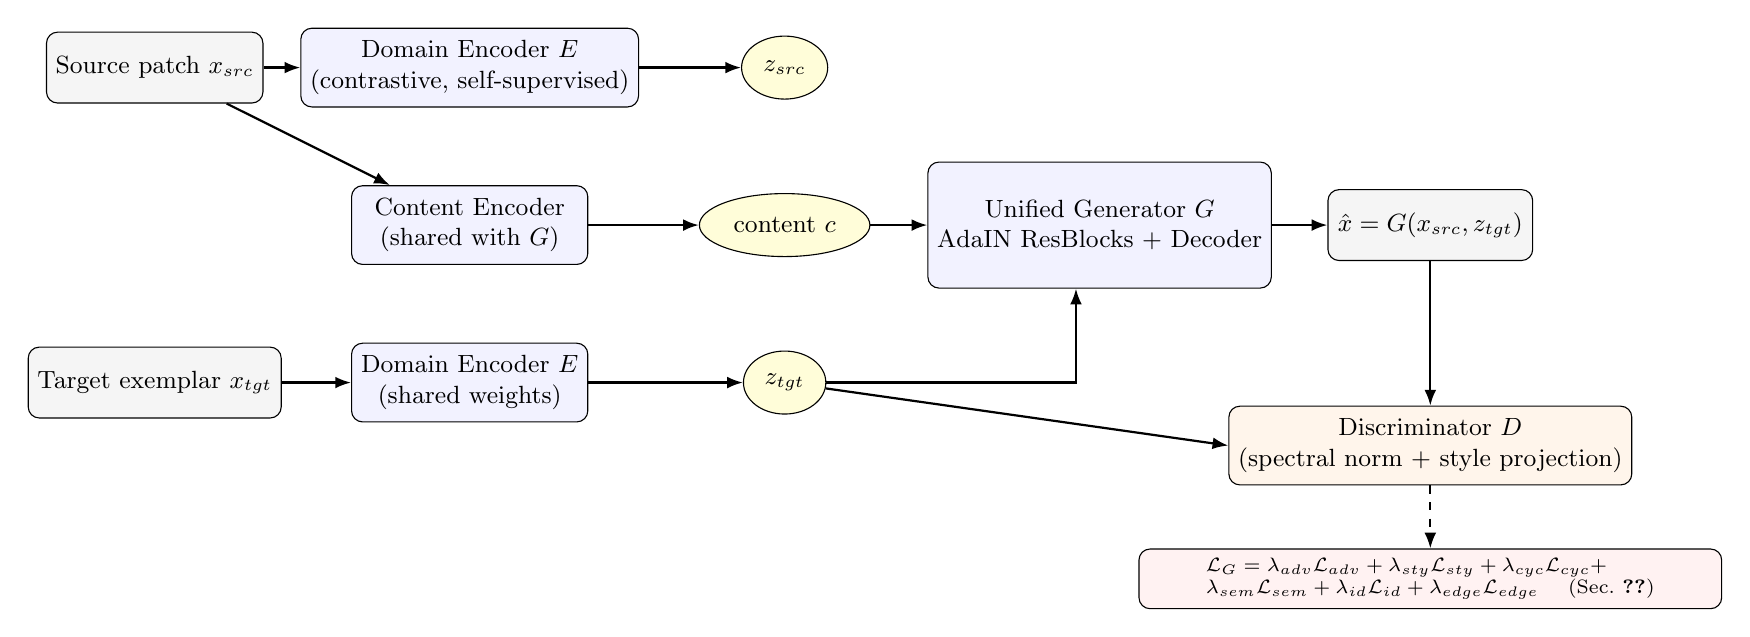
\begin{tikzpicture}[
  node distance=8mm and 10mm,
  box/.style={draw, rounded corners, align=center, minimum height=1.0cm, font=\small, fill=blue!5},
  data/.style={draw, rounded corners, align=center, minimum height=0.9cm, font=\small, fill=gray!8},
  vec/.style={draw, ellipse, align=center, minimum height=0.8cm, font=\small, fill=yellow!15},
  lossbox/.style={draw, rounded corners, align=left, font=\scriptsize, fill=red!5},
  arr/.style={-{Latex[length=2mm]}, thick}
]
  \node[data]                              (xsrc) at (0,6)    {Source patch $x_{src}$};
  \node[data]                              (xtgt) at (0,2)    {Target exemplar $x_{tgt}$};

  \node[box, minimum width=3.0cm]          (E1)   at (4.0,6)  {Domain Encoder $E$\\(contrastive, self-supervised)};
  \node[box, minimum width=3.0cm]          (CE)   at (4.0,4)  {Content Encoder\\(shared with $G$)};
  \node[box, minimum width=3.0cm]          (E2)   at (4.0,2)  {Domain Encoder $E$\\(shared weights)};

  \node[vec]                               (zsrc) at (8.0,6)  {$z_{src}$};
  \node[vec]                               (c)    at (8.0,4)  {content $c$};
  \node[vec]                               (ztgt) at (8.0,2)  {$z_{tgt}$};

  \node[box, minimum width=3.2cm, minimum height=1.6cm] (G) at (12.0,4) {Unified Generator $G$\\AdaIN ResBlocks + Decoder};

  \node[data, minimum width=2.6cm]         (xfake) at (16.2,4) {$\hat{x} = G(x_{src}, z_{tgt})$};

  \node[box, fill=orange!8, minimum width=3.0cm] (D) at (16.2,1.2) {Discriminator $D$\\(spectral norm + style projection)};

  \draw[arr] (xsrc) -- (E1);
  \draw[arr] (xsrc) -- (CE);
  \draw[arr] (xtgt) -- (E2);
  \draw[arr] (E1) -- (zsrc);
  \draw[arr] (CE) -- (c);
  \draw[arr] (E2) -- (ztgt);
  \draw[arr] (c) -- (G);
  \draw[arr] (ztgt.east) -| ([xshift=-3mm]G.south);
  \draw[arr] (G) -- (xfake);
  \draw[arr] (xfake) -- (D);
  \draw[arr] (ztgt) -- (D.west);

  \node[lossbox, below=8mm of D, minimum width=7.4cm] (losses) {
    $\mathcal{L}_G = \lambda_{adv}\mathcal{L}_{adv} + \lambda_{sty}\mathcal{L}_{sty} + \lambda_{cyc}\mathcal{L}_{cyc} +$\\
    $\lambda_{sem}\mathcal{L}_{sem} + \lambda_{id}\mathcal{L}_{id} + \lambda_{edge}\mathcal{L}_{edge}$ \quad (Sec.~\ref{sec:objective})
  };
  \draw[arr, dashed] (D.south) -- (losses.north);
\end{tikzpicture}}
\caption{Simplified architecture of the two components reported here: the self-supervised domain encoder $E$ (Sec.~\ref{sec:encoder}) and the AdaIN-conditioned generator $G$ with projection discriminator $D$ (Sec.~\ref{sec:generator}). The source embedding $z_{src}$ is reused in two further passes through $G$, omitted for clarity, for the cycle and identity losses of Sec.~\ref{sec:objective}.}
\label{fig:architecture}
\end{figure*}

The two components that are addressed in this paper are shown in Fig.~\ref{fig:architecture}. A domain encoder $E$ is used to project an unlabeled image patch to a continuous style embedding, a content encoder $G$ is used as the downsampling path of the generator to extract a domain-invariant spatial content code, and a unified generator $G$ is used to combine the content of a source patch with the embedding of a target patch to generate a translation, which is then evaluated by a projection discriminator $D$.

\subsection{Self-Supervised Continuous Domain Encoder}
\label{sec:encoder}
This is achieved by the encoder $E_\theta$ which maps an $H \times W$ patch containing $C$ channels (4 in this implementation, corresponding to 3 optical channels and 1 auxiliary channel, see Sec.~\ref{sec:dataset}) to a continuous embedding $z \in \mathbb{R}^{64}$. The network is composed of an input-adapter convolution, followed by three stride-2 convolutional blocks (Conv--InstanceNorm--LeakyReLU) to gradually reduce the spatial resolution, but expand the channel width, followed by a squeeze-and-excitation (SE) block~\cite{hu2018senet} which recalibrates the responses channel-wise.

Instead of pooling to a class score, the encoder calculates two types of statistics, the first-order mean $\mu$ and the second-order standard deviation $\sigma$ of the final feature map, representing the radiometric and textural style of the patch, respectively, without relying on spatial content:
\begin{equation}
\mu_c = \frac{1}{HW}\sum_{i,j} h_{c,i,j}, \qquad
\sigma_c = \sqrt{\frac{1}{HW}\sum_{i,j}(h_{c,i,j}-\mu_c)^2 + \epsilon}
\label{eq:stats}
\end{equation}
where $h$ is the feature map after the SE block. The concatenated statistics $[\mu;\sigma]$ (optionally fused with a projected acquisition-angle feature when angle metadata is available, unused in the sensor-only experiment reported here) are passed through a multilayer perceptron projection head and L2-normalized onto the unit hypersphere:
\begin{equation}
z = \frac{f_\phi([\mu;\sigma])}{\lVert f_\phi([\mu;\sigma]) \rVert_2}, \qquad z \in \mathbb{R}^{64}.
\label{eq:embed}
\end{equation}

The encoder is pretrained with no domain labels using a contrastive pretext task in the style of InfoNCE~\cite{oord2018cpc}. Two independently augmented views ($z_1, z_2$) of the same patch (random flips and 90\textdegree{} rotations) are treated as a positive pair, and all other patches in the training batch act as negatives:
\begin{equation}
\mathcal{L}_{con} = -\frac{1}{2B}\sum_{i=1}^{B}\Big[
\log\frac{e^{\,z_{1,i}\cdot z_{2,i}/\tau}}{\sum_{j} e^{\,z_{1,i}\cdot z_{2,j}/\tau}}
+
\log\frac{e^{\,z_{2,i}\cdot z_{1,i}/\tau}}{\sum_{j} e^{\,z_{2,i}\cdot z_{1,j}/\tau}}
\Big]
\label{eq:infonce}
\end{equation}
where $B$ is the batch size and $\tau$ is a temperature hyperparameter. Because positives and negatives come from augmentation rather than sensor labels, no supervision of domain identity is used, and any patch can be projected into the same continuous space at inference time.

\subsection{Unified Conditional Generator}
\label{sec:generator}
The generator $G_\psi$ takes a source patch $x_{src}$ and a target embedding $z_{tgt}$ (produced by the frozen encoder $E$ on a target-domain exemplar) and synthesizes a translated patch $\hat{x} = G_\psi(x_{src}, z_{tgt})$. A single generator instance is shared across all domains: the target style is entirely determined by $z_{tgt}$, so translation into any domain the encoder can embed -- rather than only domains enumerated at training time -- requires no architectural change or additional parameters.

The content path follows an encoder-bottleneck-decoder design in the spirit of StarGAN~v2~\cite{choi2020starganv2}, adapted to be label-free. A content encoder with reflection-padded convolutions and instance normalization downsamples $x_{src}$ to a domain-invariant content code $c = \mathrm{Enc}_c(x_{src})$. This code is passed through four residual blocks modulated by Adaptive Instance Normalization (AdaIN)~\cite{huang2017adain}, which injects the target style at every block:
\begin{equation}
\mathrm{AdaIN}(h, z) = \gamma(z)\cdot\frac{h - \mu(h)}{\sigma(h)} + \beta(z)
\label{eq:adain}
\end{equation}
where $\mu(h), \sigma(h)$ are the per-channel instance statistics of the intermediate feature map $h$, and $\gamma(z) = W_\gamma z + b_\gamma$, $\beta(z) = W_\beta z + b_\beta$ are affine parameters regressed from the continuous embedding. The decoder mirrors the encoder with two AdaIN-modulated upsampling stages; bilinear (rather than nearest-neighbor or transposed-convolution) upsampling is used to avoid checkerboard artifacts, followed by a reflection-padded output convolution with a $\tanh$ activation.

\subsection{Discriminator with Continuous Style Projection}
The discriminator $D_\xi$ is a multi-scale PatchGAN with spectral normalization~\cite{miyato2018spectral} applied to every convolutional layer, which stabilizes adversarial training by bounding the Lipschitz constant of each layer. In addition to an unconditional real/fake head, $D_\xi$ projects its intermediate features onto the conditioning embedding $z$:
\begin{equation}
D_\xi(x, z) = D_{uncond}(x) + \frac{\langle \phi(x), W_{proj}\,z\rangle}{\sqrt{d}}
\label{eq:disc}
\end{equation}
where $\phi(x)$ is the discriminator's penultimate feature map, $W_{proj}$ is a learned linear projection of the embedding, and $d$ is the feature dimension. This term penalizes translations whose visual style does not match the conditioning embedding $z$, complementing the encoder's own style-reconstruction signal (Sec.~\ref{sec:objective}).

\subsection{Composite Training Objective}
\label{sec:objective}
The generator is trained with a weighted sum of six loss terms, each targeting a specific failure mode observed in unconstrained multi-domain translation:

\emph{Adversarial loss} (least-squares GAN~\cite{mao2017lsgan}), encouraging $\hat{x}$ to be indistinguishable from real target-domain patches under the style-conditioned discriminator:
\begin{align}
\mathcal{L}_D &= \tfrac{1}{2}\mathbb{E}\big[(D_\xi(x_{tgt}, z_{tgt}) - 1)^2\big] + \tfrac{1}{2}\mathbb{E}\big[D_\xi(\hat{x}, z_{tgt})^2\big] \\
\mathcal{L}_{adv} &= \mathbb{E}\big[(D_\xi(\hat{x}, z_{tgt}) - 1)^2\big]
\label{eq:adv}
\end{align}

\emph{Style-reconstruction loss}, requiring the target style to be measurable in the output by re-encoding it:
\begin{equation}
\mathcal{L}_{sty} = \mathbb{E}\,\lVert E(\hat{x}) - z_{tgt} \rVert_1
\label{eq:sty}
\end{equation}

\emph{Cycle-consistency loss}~\cite{zhu2017cyclegan}, translating $\hat{x}$ back toward the source style and requiring recovery of the original patch, which discourages mode collapse across domains:
\begin{equation}
\mathcal{L}_{cyc} = \mathbb{E}\,\lVert G(\hat{x}, z_{src}) - x_{src} \rVert_1
\label{eq:cyc}
\end{equation}

\emph{Semantic-preservation loss}, penalizing drift in the domain-invariant content code between the source and the translation, so that geospatial layout (parcel boundaries, roads) is not altered by the style change:
\begin{equation}
\mathcal{L}_{sem} = \mathbb{E}\,\lVert \mathrm{Enc}_c(\hat{x}) - \mathrm{Enc}_c(x_{src}) \rVert_1
\label{eq:sem}
\end{equation}

\emph{Identity loss}, requiring that conditioning the generator on the source's own style leaves the patch unchanged:
\begin{equation}
\mathcal{L}_{id} = \mathbb{E}\,\lVert G(x_{src}, z_{src}) - x_{src} \rVert_1
\label{eq:id}
\end{equation}

\emph{Edge-preservation loss}, comparing Sobel gradient magnitudes between $\hat{x}$ and $x_{src}$ to keep agricultural parcel boundaries and road edges sharp:
\begin{equation}
\mathcal{L}_{edge} = \mathbb{E}\,\lVert \nabla_{Sobel}(\hat{x}) - \nabla_{Sobel}(x_{src}) \rVert_1
\label{eq:edge}
\end{equation}

The total generator objective is
\begin{align}
\mathcal{L}_G ={}& \lambda_{adv}\mathcal{L}_{adv} + \lambda_{sty}\mathcal{L}_{sty} + \lambda_{cyc}\mathcal{L}_{cyc} \notag \\
& + \lambda_{sem}\mathcal{L}_{sem} + \lambda_{id}\mathcal{L}_{id} + \lambda_{edge}\mathcal{L}_{edge}
\label{eq:total}
\end{align}
with weights listed in Table~\ref{tab:hyperparams}. The framework additionally defines a geometric (SSIM-style) preservation loss $\mathcal{L}_{geo}$, activated when either the source or target domain is an off-nadir viewing-angle domain; because the PASTIS-HD experiment reported in Sec.~\ref{sec:results} uses only sensor domains, $\mathcal{L}_{geo}$ is inactive ($\lambda_{geo}\mathcal{L}_{geo}=0$) for the results shown here.

\section{Dataset and Preprocessing}
\label{sec:dataset}
Experiments are conducted on patches that are taken from PASTIS-HD~\cite{garnot2021panoptic,astruc2024omnisat} a public benchmark of $2{,}433$ co-registered agricultural-parcel locations in France for which SAR time series from Sentinel-2 and Sentinel-1 datasets are provided, and in the HD extension a very-high-resolution image from SPOT~6/7. A conversion pipeline matches up patches by identifier and exports a $128\times128$ 4-channel tensor per modality, per location: Sentinel-2 Red, Green, Blue and near-infrared channels are kept as is; SPOT~6/7 is resized from $1280\times1280$ and provided with a synthetic near-infrared proxy channel, and the two polarizations of Sentinel-1 (VV and VH) are extended with a derived ratio and average channel, and are converted from decibel to linear units. All modalities have the range of [-1,1]. In this experiment, the first $1{,}500$ locations per domain in identifier order (the patch cap of the pipeline) is converted from three Sentinel-2 tiles. In this case, 80\% of the patches are used as training data and 20\% are held out, with 1200 used in the training set and 300 held out, meaning that all held out patches are in a single region, only slightly underrepresented in training, and the evaluation is largely on a different region. The modalities are co-registered, but not simultaneous: the first Sentinel-1 acquisition is 11 days after the first Sentinel-2 acquisition (median) and the SPOT imagery is provided from 2019. After conversion, the SAR difference channel is saturated at $+1$ for 97.9\% of its values. Random flips, rotations by 90\textdegree{} and small Gaussian radiometric noise $\sigma \sim \mathcal{U}[0, 0.01]$ are added to the training patches.

\section{Experimental Setup}
\label{sec:setup}
It is implemented in Python~3.13 with PyTorch~$\geq$2.4 and is controlled by a single command line entry point, which first trains the domain-encoder, then trains the generator and discriminator jointly. All training and evaluation were performed on the CPU of a laptop with following specification: Intel Core i7-9750H, 6 core, 7.8~GB RAM. The width of the generator and discriminator (base width 32) is kept narrow to ensure this compute is tractable for training, rather than be close to a reported baseline. For the results in Sec.~\ref{sec:results} the following hyperparameters were used, as shown in Tab.~\ref{tab:hyperparams}.

\begin{table}[t]
\centering
\caption{Training hyperparameters.}
\label{tab:hyperparams}
\begin{tabular}{@{}ll@{}}
\toprule
\textbf{Stage 1 -- Domain Encoder} & \textbf{Value} \\
\midrule
Embedding dimension $d$            & 64 \\
Optimizer                          & AdamW \\
Learning rate                      & $5\times10^{-4}$ \\
Weight decay                       & $1\times10^{-4}$ \\
Contrastive temperature $\tau$     & 0.07 \\
Epochs                             & 10 \\
\midrule
\textbf{Stage 2 -- Generator / Discriminator} & \textbf{Value} \\
\midrule
Base channel width                 & 32 \\
Residual blocks                    & 4 \\
Optimizer ($G$, $D$)               & Adam ($\beta_1{=}0.5$, $\beta_2{=}0.999$) \\
Learning rate ($G$, $D$)           & $3\times10^{-4}$ \\
LR schedule                        & Cosine annealing, $\eta_{min}{=}10^{-5}$ \\
Gradient clipping (max norm)       & 1.0 \\
Epochs                             & 12 \\
Batch size                         & 8 \\
$\lambda_{adv},\lambda_{sty},\lambda_{id}$ & 1.0 each \\
$\lambda_{sem}$, $\lambda_{edge}$  & 2.0 each \\
$\lambda_{cyc}$                    & 10.0 \\
\bottomrule
\end{tabular}
\end{table}

\section{Results and Discussion}
\label{sec:results}
All results are on the 300 withheld patches per domain with a constant protocol and are only a single measurement from one trained model. Target domains are L2-normalized mean of the embedding of 1200 patches in the target domain, which are the \emph{centroid} of the domain (the training patches are used in the embedding process, but not for the evaluation step). The images are rescaled to $[0,1]$ against the co-registered real target patch, having two reference baselines: ``Copy'' for the untranslated source patch, and ``Const.'' for the constant image that corresponds to the mean of the target domain.

\subsection{Domain encoder (Objective~1)}
Table~\ref{tab:enc} summarizes the encoder. It achieves a solution to its contrastive task on held-out patches (loss 0.24 compared to 2.08 with an uninformative embedding; 88.2\% top-1 retrieval of the second view on 900 patches), while its embeddings are uniformly distributed over the hypersphere rather than in three concentrated clusters. They describe the sensor moderately: 65.8\% of held out patches are correctly assigned to the sensor by the nearest centroid as compared with 33.3\% randomly; the sensors overlap (silhouette coefficient 0.11); effective dimensionality is about 4. The co-registered patch of another sensor is retrieved at chance level, which means that the embedding does not contain information about the scene that is shared across sensors. One possible reason (not tested) is that instance discrimination does not include a term to group the patches of one sensor, and that proximity-based positive pairs as planned in the project plan were not used.

\begin{table}[t]
\centering
\caption{Domain encoder on 300 held-out patches per domain (S2: Sentinel-2).}
\label{tab:enc}
\begin{tabular}{@{}lc@{}}
\toprule
\textbf{Measurement} & \textbf{Result} \\
\midrule
Held-out InfoNCE loss (batch 8; chance 2.08)        & 0.24 \\
Top-1 instance retrieval among 900 patches          & 88.2\% \\
Nearest-centroid domain accuracy (chance 33.3\%)    & 65.8\% \\
\quad recall S2 / SPOT / SAR                        & 62.7 / 74.3 / 60.3\% \\
5-nearest-neighbor domain accuracy                  & 63.7\% \\
Cosine similarity within / between domains          & 0.32 / 0.04 \\
Silhouette coefficient (cosine distance)            & 0.11 \\
Participation ratio (of 64 dimensions)              & 3.85 \\
Same-location retrieval across sensors, top-1       & 0.3\% (chance 0.3\%) \\
\bottomrule
\end{tabular}
\end{table}

\subsection{Conditional generator (Objective~2)}
\begin{figure*}[t]
\centering
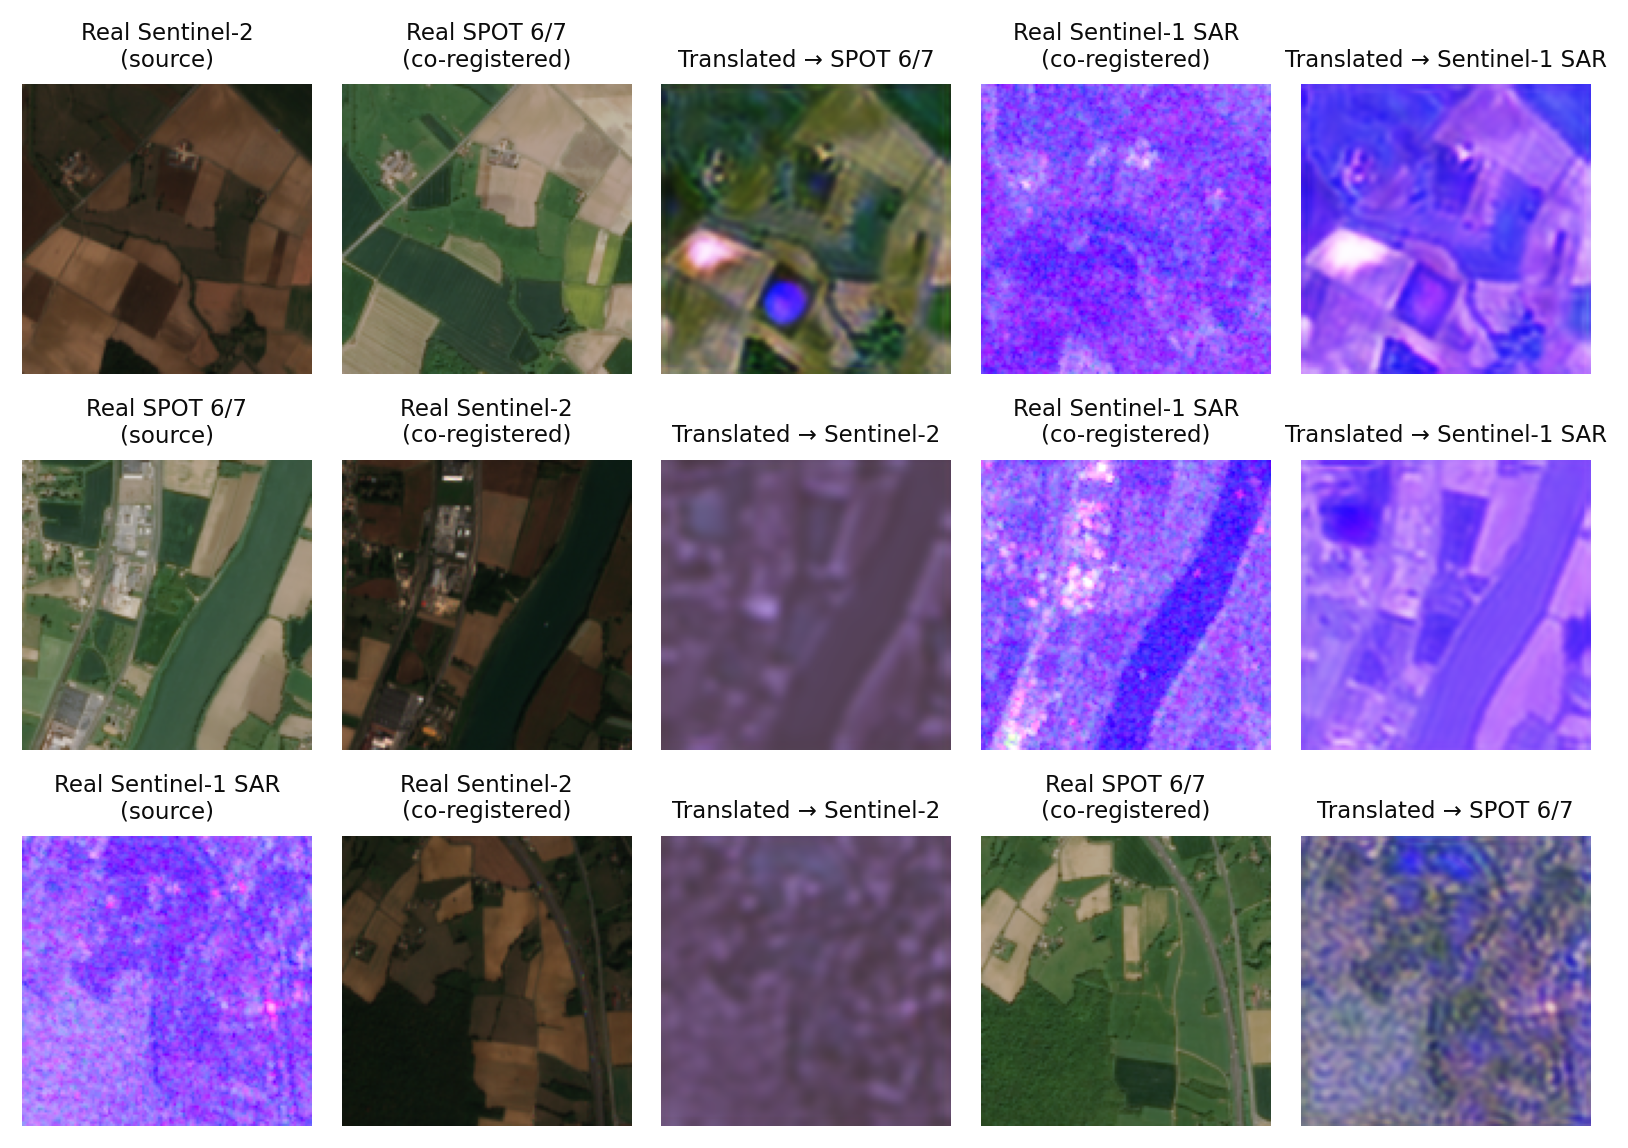
\includegraphics[width=0.7\textwidth]{figures/fig_paired_translation.png}
\caption{Translations of one held-out patch per source domain (first column of each row) into the two other domains, next to the real co-registered patch of each target domain. The style is the centroid embedding of the target domain, and the patches were chosen by a fixed random seed before inspection. Sentinel-1 patches are displayed as VV, VH, and the saturated difference channel in red, green, and blue.}
\label{fig:paired}
\end{figure*}

\begin{table}[t]
\centering
\caption{Translation into each target on held-out patches. PSNR (dB) against the co-registered real target patch for the translation, for the copied source (Copy) and for a constant target-mean image (Const.); Style is the share of outputs that the encoder assigns to the target domain; Edge is the edge-map correlation with the source.}
\label{tab:gen}
\footnotesize
\setlength{\tabcolsep}{3.5pt}
\begin{tabular}{@{}lccccc@{}}
\toprule
\textbf{Pair} & \textbf{Transl.} & \textbf{Copy} & \textbf{Const.} & \textbf{Style} & \textbf{Edge} \\
\midrule
S2 $\rightarrow$ SPOT   & 14.6 & 13.1 & 17.2 & 57\% & 0.82 \\
S2 $\rightarrow$ SAR    & 14.6 & 5.7 & 20.5 & 18\% & 0.87 \\
SPOT $\rightarrow$ S2   & 13.5 & 13.1 & 17.8 & 29\% & 0.71 \\
SPOT $\rightarrow$ SAR  & 16.8 & 7.4 & 20.5 & 80\% & 0.82 \\
SAR $\rightarrow$ S2    & 13.3 & 5.7 & 17.8 & 12\% & 0.94 \\
SAR $\rightarrow$ SPOT  & 13.0 & 7.4 & 17.2 & 45\% & 0.92 \\
\bottomrule
\end{tabular}
\end{table}

The style vector is used: the PSNR for the source to translation is higher than for the source to the real target domain (by 3.3 to 7.6~dB) for 5 of 6 pairs, and parcels are still recognizable in the figure, even though the road is not. The target radiometry is not reproduced: the constant image is correlated better with the real target patch than the translation for all 6 pairs (by 2.6 to 5.9~dB; the correlation is always higher than 0.61, better for pairs involving SAR than for others), the encoder assigns the outputs to the target domain in only 12\% to 80\% of the cases, and translations into Sentinel-2 are a blurred purple-gray haze whose channel means are equal within 0.001 for all 3 sources, and much brighter than real Sentinel-2 patches (by The identity mapping of Sentinel-2 is also not very well reproduced (13.7~dB, while for SPOT and SAR 20.3~dB and 24.3~dB, respectively); Sentinel-2 is the least strong of the generator both as source and as target. The different modalities acquired at different times constrained the degree to which the pixels may be matched, but did not account for the poorer transmission of a constant image.

The style space of the two points was sampled by interpolating between the two domain centroids, $z(\alpha)=(1-\alpha)\bar z_a+\alpha\bar z_b$ with the points renormalized to unit length, for 300 sets of source patches. The two pairs involving SAR resulted in a smooth change in output, close to linear (linearity ratio 0.91 and 0.96, monotone for 96\% and 100\% of the patches, respectively). The change is 10\% smaller for Sentinel-2 and SPOT, and only the first step ($0<\alpha<0.25$) contains the majority of the change 89\% of the patches, with only 41\% of them being monotone. There are 1.59~M parameters for the generator and 0.89~M for the encoder, and the CPU takes approximately 84~ms for a translation per patch.

Fig.~\ref{fig:interp} shows this interpolation for one held-out SPOT~6/7 source patch.

\begin{figure}[t]
\centering
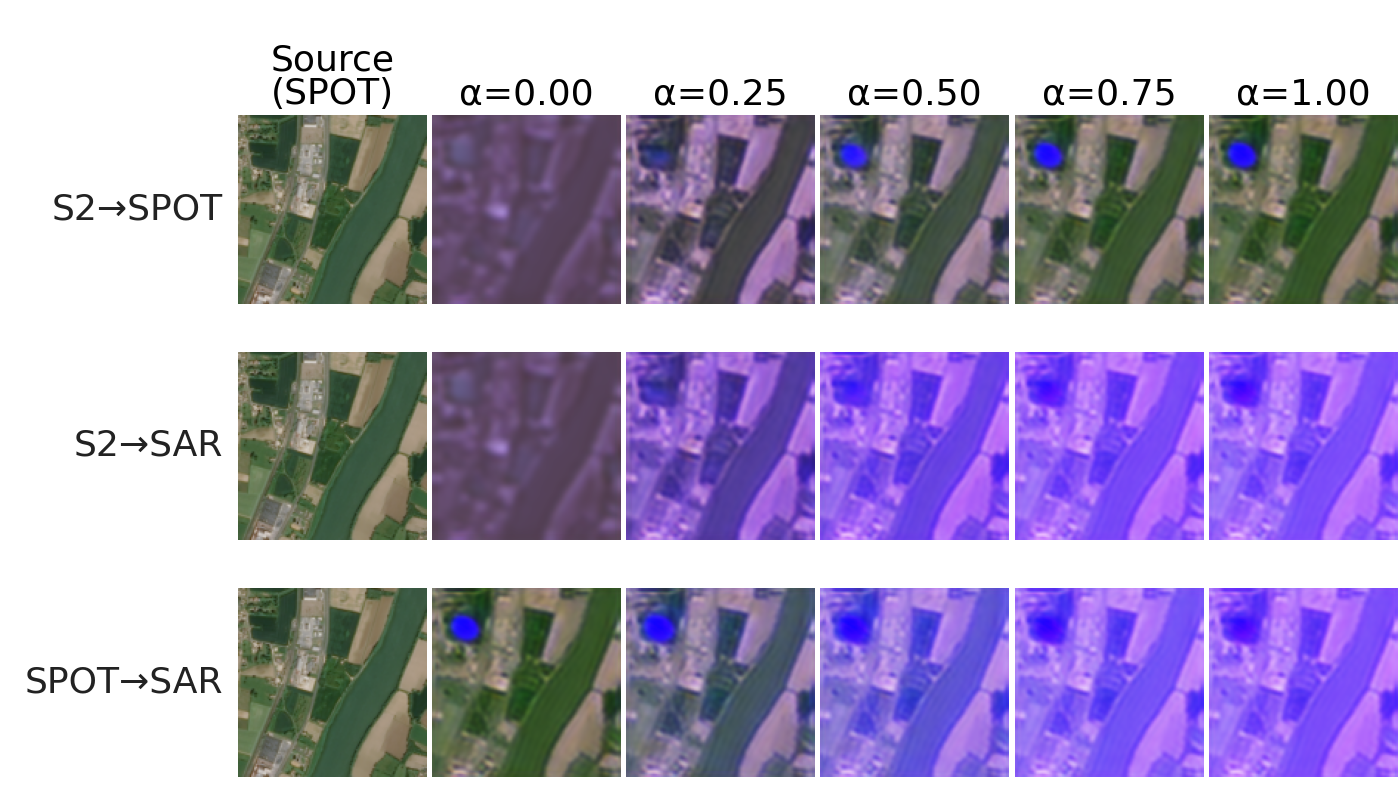
\includegraphics[width=\columnwidth]{figures/fig_interp_compact.png}
\caption{Interpolation of the style vector between two domain centroids, $z(\alpha)=(1-\alpha)\bar z_a+\alpha\bar z_b$ renormalized to unit length, applied to one held-out SPOT~6/7 source patch (first column). Each row is a pair of domains $a \rightarrow b$ and $\alpha$ runs from the style of $a$ ($\alpha=0$) to the style of $b$ ($\alpha=1$). The patch was chosen by a fixed random seed before inspection.}
\label{fig:interp}
\end{figure}

The architectural objectives of Table~\ref{tab:gap} are achieved: there is no labeling of the domain, a single generator for all the ordered pairs of three domains, and a continuous 64-dimensional domain code. None of the cited methods were trained on the same data as used for this work, and the numbers published for these methods are from other data and tasks, so any comparison to the quality of the result is not warranted, and no claim is made that the approach is better than SS(DA)$^2$, StarGAN~v2, or any of the other methods.

\section{Limitations}
\label{sec:limitations}
The above results have some restrictions. First, the held-out patches are from one Sentinel-2 tile, and the training set is largely from two other tiles, and so the results are a blend of model quality and a shift towards a different region; domain centroids are from different regions to the patches they're applied to. Second, there is no simultaneous modality, limiting the ability to agree at the pixel level with the co-registered reference, and there are artifacts in the preprocessing (saturated SAR channel and synthetic fourth SPOT channel). Third, for each model, the training was performed only once on a CPU with only 12 epochs of the generator and 10 epochs of the encoder (Sec.~\ref{sec:setup}), and the training loops were not seeded, no run-to-run variation was tested, no ablation of the six generator losses was performed, and no other method of translation was trained on the same data. Fourth, PSNR and SSIM are used for the degree of agreement with a co-registered image, not for realism, and the rate of style transfer is evaluated by the same encoder used for conditioning the generator. Fifth, only three sensor domains, one geographic setting and 1,500 of 2,433 locations were utilized; the larger MSC-France corpus that was foreseen forencoder pretraining and the angle-conditioning were not used. Finally, generalisation of unseen sensor pairs and downstream accuracy are not assessed.

\section{Conclusion and Future Work}
The proposed framework was a novel multi-domain self-supervised adaptation framework for satellite-based image data, which consisted of two main components: a contrastive domain encoder for learning label-free, continuous embeddings of the sensor style of the images, and an AdaIN-conditioned generator for generating an image in an arbitrary target style, given a source patch and its learned embedding from the domain encoder. The framework has the potential to comply with the design goals at the architectural level: No domain labels, one model for all ordered domain pairs, a continuous domain code, trained on real PASTIS-HD imagery (Sentinel-2, SPOT~6/7, Sentinel-1 SAR). There is a limited measured quality: the encoder identifies the sensor moderately (65.8\% vs 33.3\% chance) and the generator preserves the structure of the scene and uses the style vector, but cannot reproduce the radiometry of the measured sensor; translations into Sentinel-2 do not work.

Future work will involve (i) replacing the augmented-view positives with sensor-aware positive pairs based on spatial and temporal proximity and pretraining on a larger corpus MSC-France; (ii) fixing data issues found here, including all PASTIS-HD patches, a tile-stratified split and temporally matched acquisitions, a non-saturating SAR channel; (iii) training wider networks longer on a GPU with seeded runs, loss ablations and same-data baselines; and (iv) testing leave-one-domain-pair-out and zero-shot (SpaceNet~6) generalization and downstream crop classification and segmentation.

\bibliographystyle{IEEEtran}
\bibliography{references}

\end{document}
"
% Camera-ready build (authors shown): pdflatex main.tex
\ifdefined\ANON
\author{
\IEEEauthorblockN{Anonymous Authors}
\IEEEauthorblockA{Anonymous Affiliation}
}
\else
\author{
\IEEEauthorblockN{Shivangi\textsuperscript{1}, Benedict Tephila M.\textsuperscript{2}, Naveen J.\textsuperscript{3}}
\IEEEauthorblockA{
Department of Computer Science and Engineering \\
CHRIST (Deemed to be University), Bangalore -- 560029, India \\
\textsuperscript{1}shivangi.a@mtech.christuniversity.in,
\textsuperscript{2}benedict.tephila@christuniversity.in,
\textsuperscript{3}naveen.j@christuniversity.in}
}
\fi

\maketitle

\begin{abstract}
The performance of deep learning models trained for the analysis of satellite images suffers when the same land-cover classes are captured by a different sensor, at a different season, or in a different region. Current domain-adaptation techniques typically require labeled target data, a fixed domain library, or both, but these are hard to obtain with evolving and expanding multi-sensor archives. Firstly, we present a continuous domain encoder that produces a label-free style embedding from unlabeled multi-sensor patches through the use of a contrastive (InfoNCE) pretext task, and secondly, we introduce a unified conditional generator that creates a style conditioned transformation of the content of the source patch into an arbitrary style of the target domain by learning a style embedding as a continuous latent space rather than a discrete class label. Both networks trained on 1,200 patches per sensor provided by PASTIS-HD (Sentinel-2, SPOT~6/7, Sentinel-1 SAR) and tested on 300 held-out patches per sensor from a region that is mostly different. The encoder successfully completes its pretext task, but recognises the sensor with only some success (65.8\% as opposed to 33.3\% chance). The generator maintains the scene structure and performs well on the pairs that contain SAR, but does not reproduce the radiometry of the target sensor: a constant image is closer to the actual target patch than a translation, and translated images end up as a source-independent color cast, when SAR is present in one of the pairs. This paper does not include generalization to unseen sensor pairs, nor does it include downstream accuracy.
\end{abstract}

\begin{IEEEkeywords}
domain adaptation, self-supervised learning, generative adversarial networks, contrastive learning, multi-sensor satellite imagery, image-to-image translation
\end{IEEEkeywords}

\section{Introduction}

Satellite remote sensing has now evolved from one single mission to a constellation of optical and radar satellites, seeing the Earth's surface together and in succession, such as Sentinel-2, Landsat, SPOT and a growing number of commercial very-high-resolution (VHR) and synthetic aperture radar (SAR) satellites. The use of deep learning models for land-cover classification, crop mapping and change detection has been increasingly placed on the ability to perform on this multi-sensor heterogeneous archive, as opposed to the single sensor they were trained on.

It is hard to achieve this cross-sensor requirement in practice. These include different radiometric calibration, spectral response, spatial resolution, and noise properties for each sensor, which vary from atmospheric haze and calibration drift in optical imagery to speckle noise and incidence-angle-dependent backscatter in SAR. Consequently, a model trained with the statistics from one sensor may exhibit a dramatic decrease in accuracy when applied to another sensor, even when the land-cover classes are the same. Modeling often requires the adaptation to a new domain with little or no target domain labeled data because of the high cost of acquiring and annotating imagery from all sensors of interest.

The current methods can be classified into two families. Satellite-specific methods, like multi-source standardization~\cite{tasar2020standardgan} normalize translation on a discrete domain identity that is manually assigned to each satellite and are claimed to have difficulty with unseen combinations of domains. However, self-supervised methods like SS(DA)$^2$~\cite{zhang2023ssdada} do not require labels or an explicit domain boundary and only translate between two satellites at a time, meaning that a new method must be developed for each new pair of satellites. In the general image-translation literature, StarGAN~\cite{choi2018stargan} and StarGAN~v2~\cite{choi2020starganv2} integrate a multitude of domains into a single generator, with StarGAN~v2 additionally using a continuous style code, and performing regular evaluations on natural images. Diffusion-based translators~\cite{vinholi2024multisensor,kieu2025universal} are more faithful but work on discrete domain sets, with higher inference cost.

The combination of label-free training, a continuous (discretely labeled is not the only option) representation of the domain and a single generator that can translate into an arbitrary target style is not yet explicitly provided in the literature for satellite images. It is the motivation for the present work to fill this gap.

The first two properties are addressed by further developing the pairwise approach of the SS(DA)$^2$ paradigm to a continuous, StarGAN~v2-style unified generator without the need for any domain-specific conditioning: A domain encoder produces a uniform embedding of the domain characteristics of each patch, and a single generator, modulated by the embedding through the use of AdaIN, maps a source patch to the domain of any target patch's embedding. These two components are designed, implemented, and evaluated using held-out data, which is not covered by this paper.

This paper makes the following contributions:
\begin{itemize}
\item A self-supervised contrastive domain encoder to generate label-free, continuous embeddings of sensor/style features from unlabeled multi-sensor patches.
A single AdaIN-modulated conditional generator conditioned on this embedding, instead of a discrete domain code, so no retraining per domain pair is required for the translation to an arbitrary target style.
An objective for six terms of training that maintains the geospatial content while changing the style of the content.
\item held out evaluation on real PASTIS-HD data that reports what works (label-free continuous embeddings, structure preserving, style conditioned translation) and what doesn't (moderate sensor information in the embedding, target radiometry not reproduced).
\end{itemize}

\section{Related Work}

\subsection{Domain Adaptation for Satellite Imagery}
StandardGAN~\cite{tasar2020standardgan} is used to standardize each source domain towards a common reference for semantic segmentation of multi-source VHR satellite images towards the common reference. It works on a set of discrete and enumerated domains, and according to the report of its authors, it has trouble maintaining the content of the images and it has poor generalisation ability with respect to sensor combinations not encountered at the time of standardisation. SS(DA)$^2$~\cite{zhang2023ssdada} does not require labeled target data or the domain boundary: a contrastive, domain-agnostic GAN translates between two satellite domains with unlabeled images. The downside to this, and what is being solved here, is that it is pairwise: each model can accommodate only two satellites.

\subsection{Multi-Domain Image-to-Image Translation}
StarGAN~\cite{choi2018stargan} combined multi-domain translation into a single generator, and used a discrete one-hot domain vector as the condition. It is replaced in StarGAN~v2~\cite{choi2020starganv2} by a continuous style code from a mapping network or style encoder fed into AdaIN~\cite{huang2017adain} and it is evaluated on natural image datasets, using realism metrics (e.g., FID), and not on satellite imagery. Multi-sensor optical image translation~\cite{vinholi2024multisensor} and universal multi-domain routing~\cite{kieu2025universal} are both based on diffusion and enhance fidelity, but the router still chooses from a discrete set of domain experts and iterative sampling is more expensive than one feed-forward GAN pass, especially for large mosaics of satellites.

\section{Research Gap and Motivation}
The most similar methods are compared to the properties targeted here in Table~\ref{tab:gap}. SS(DA)$^2$ is label-free and pairwise while StarGAN~v2 is continuous domain representation and supervised discrete domain identity at training time, and designed for remote sensing; StandardGAN is designed for satellite imagery and requires discrete domain identity. All the methods reviewed here did not accept labels and used a continuous domain without a generator specifically designed for and tested on satellite images. This project's goals, ~1 and ~2, are specifically aimed at this combination: Continuous domain encoder without labels, and a single generator conditioned on its embedding.

\begin{table}[t]
\centering
\caption{Qualitative comparison of properties relevant to the identified research gap.}
\label{tab:gap}
\resizebox{\linewidth}{!}{%
\begin{tabular}{@{}lccc@{}}
\toprule
\textbf{Method} & \textbf{Label-free} & \textbf{Continuous domain repr.} & \textbf{Satellite-specific} \\
\midrule
StandardGAN~\cite{tasar2020standardgan}    & \ding{55} & \ding{55} & \ding{51} \\
SS(DA)$^2$~\cite{zhang2023ssdada}          & \ding{51} & \ding{55} (pairwise) & \ding{51} \\
StarGAN~\cite{choi2018stargan}             & \ding{55} & \ding{55} & \ding{55} \\
StarGAN~v2~\cite{choi2020starganv2}        & \ding{55} & \ding{51} & \ding{55} \\
\textbf{Proposed (Objectives 1--2)}        & \ding{51} & \ding{51} & \ding{51} \\
\bottomrule
\end{tabular}}
\end{table}

\section{Proposed Methodology}

\begin{figure*}[t]
\centering
\resizebox{\textwidth}{!}{%
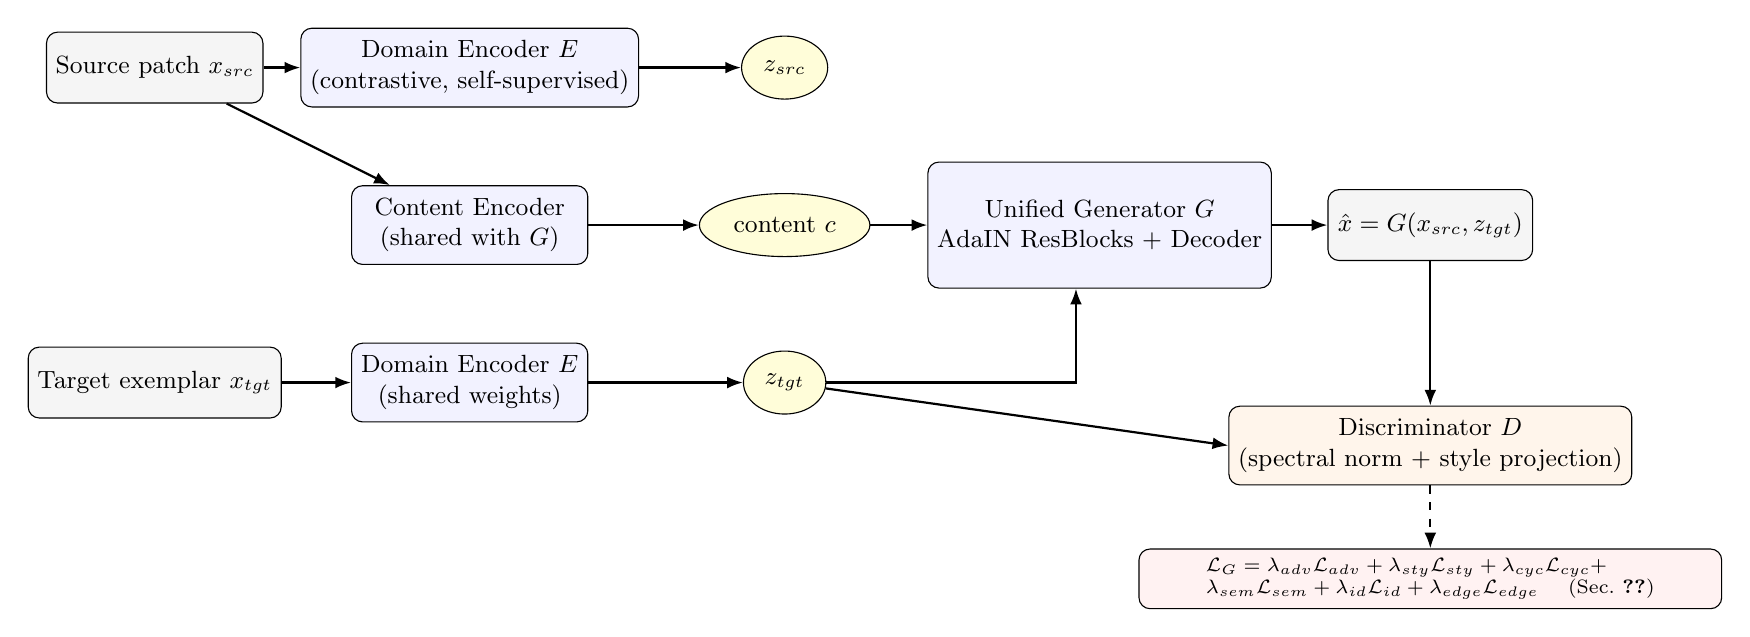
\begin{tikzpicture}[
  node distance=8mm and 10mm,
  box/.style={draw, rounded corners, align=center, minimum height=1.0cm, font=\small, fill=blue!5},
  data/.style={draw, rounded corners, align=center, minimum height=0.9cm, font=\small, fill=gray!8},
  vec/.style={draw, ellipse, align=center, minimum height=0.8cm, font=\small, fill=yellow!15},
  lossbox/.style={draw, rounded corners, align=left, font=\scriptsize, fill=red!5},
  arr/.style={-{Latex[length=2mm]}, thick}
]
  \node[data]                              (xsrc) at (0,6)    {Source patch $x_{src}$};
  \node[data]                              (xtgt) at (0,2)    {Target exemplar $x_{tgt}$};

  \node[box, minimum width=3.0cm]          (E1)   at (4.0,6)  {Domain Encoder $E$\\(contrastive, self-supervised)};
  \node[box, minimum width=3.0cm]          (CE)   at (4.0,4)  {Content Encoder\\(shared with $G$)};
  \node[box, minimum width=3.0cm]          (E2)   at (4.0,2)  {Domain Encoder $E$\\(shared weights)};

  \node[vec]                               (zsrc) at (8.0,6)  {$z_{src}$};
  \node[vec]                               (c)    at (8.0,4)  {content $c$};
  \node[vec]                               (ztgt) at (8.0,2)  {$z_{tgt}$};

  \node[box, minimum width=3.2cm, minimum height=1.6cm] (G) at (12.0,4) {Unified Generator $G$\\AdaIN ResBlocks + Decoder};

  \node[data, minimum width=2.6cm]         (xfake) at (16.2,4) {$\hat{x} = G(x_{src}, z_{tgt})$};

  \node[box, fill=orange!8, minimum width=3.0cm] (D) at (16.2,1.2) {Discriminator $D$\\(spectral norm + style projection)};

  \draw[arr] (xsrc) -- (E1);
  \draw[arr] (xsrc) -- (CE);
  \draw[arr] (xtgt) -- (E2);
  \draw[arr] (E1) -- (zsrc);
  \draw[arr] (CE) -- (c);
  \draw[arr] (E2) -- (ztgt);
  \draw[arr] (c) -- (G);
  \draw[arr] (ztgt.east) -| ([xshift=-3mm]G.south);
  \draw[arr] (G) -- (xfake);
  \draw[arr] (xfake) -- (D);
  \draw[arr] (ztgt) -- (D.west);

  \node[lossbox, below=8mm of D, minimum width=7.4cm] (losses) {
    $\mathcal{L}_G = \lambda_{adv}\mathcal{L}_{adv} + \lambda_{sty}\mathcal{L}_{sty} + \lambda_{cyc}\mathcal{L}_{cyc} +$\\
    $\lambda_{sem}\mathcal{L}_{sem} + \lambda_{id}\mathcal{L}_{id} + \lambda_{edge}\mathcal{L}_{edge}$ \quad (Sec.~\ref{sec:objective})
  };
  \draw[arr, dashed] (D.south) -- (losses.north);
\end{tikzpicture}}
\caption{Simplified architecture of the two components reported here: the self-supervised domain encoder $E$ (Sec.~\ref{sec:encoder}) and the AdaIN-conditioned generator $G$ with projection discriminator $D$ (Sec.~\ref{sec:generator}). The source embedding $z_{src}$ is reused in two further passes through $G$, omitted for clarity, for the cycle and identity losses of Sec.~\ref{sec:objective}.}
\label{fig:architecture}
\end{figure*}

The two components that are addressed in this paper are shown in Fig.~\ref{fig:architecture}. A domain encoder $E$ is used to project an unlabeled image patch to a continuous style embedding, a content encoder $G$ is used as the downsampling path of the generator to extract a domain-invariant spatial content code, and a unified generator $G$ is used to combine the content of a source patch with the embedding of a target patch to generate a translation, which is then evaluated by a projection discriminator $D$.

\subsection{Self-Supervised Continuous Domain Encoder}
\label{sec:encoder}
This is achieved by the encoder $E_\theta$ which maps an $H \times W$ patch containing $C$ channels (4 in this implementation, corresponding to 3 optical channels and 1 auxiliary channel, see Sec.~\ref{sec:dataset}) to a continuous embedding $z \in \mathbb{R}^{64}$. The network is composed of an input-adapter convolution, followed by three stride-2 convolutional blocks (Conv--InstanceNorm--LeakyReLU) to gradually reduce the spatial resolution, but expand the channel width, followed by a squeeze-and-excitation (SE) block~\cite{hu2018senet} which recalibrates the responses channel-wise.

Instead of pooling to a class score, the encoder calculates two types of statistics, the first-order mean $\mu$ and the second-order standard deviation $\sigma$ of the final feature map, representing the radiometric and textural style of the patch, respectively, without relying on spatial content:
\begin{equation}
\mu_c = \frac{1}{HW}\sum_{i,j} h_{c,i,j}, \qquad
\sigma_c = \sqrt{\frac{1}{HW}\sum_{i,j}(h_{c,i,j}-\mu_c)^2 + \epsilon}
\label{eq:stats}
\end{equation}
where $h$ is the feature map after the SE block. The concatenated statistics $[\mu;\sigma]$ (optionally fused with a projected acquisition-angle feature when angle metadata is available, unused in the sensor-only experiment reported here) are passed through a multilayer perceptron projection head and L2-normalized onto the unit hypersphere:
\begin{equation}
z = \frac{f_\phi([\mu;\sigma])}{\lVert f_\phi([\mu;\sigma]) \rVert_2}, \qquad z \in \mathbb{R}^{64}.
\label{eq:embed}
\end{equation}

The encoder is pretrained with no domain labels using a contrastive pretext task in the style of InfoNCE~\cite{oord2018cpc}. Two independently augmented views ($z_1, z_2$) of the same patch (random flips and 90\textdegree{} rotations) are treated as a positive pair, and all other patches in the training batch act as negatives:
\begin{equation}
\mathcal{L}_{con} = -\frac{1}{2B}\sum_{i=1}^{B}\Big[
\log\frac{e^{\,z_{1,i}\cdot z_{2,i}/\tau}}{\sum_{j} e^{\,z_{1,i}\cdot z_{2,j}/\tau}}
+
\log\frac{e^{\,z_{2,i}\cdot z_{1,i}/\tau}}{\sum_{j} e^{\,z_{2,i}\cdot z_{1,j}/\tau}}
\Big]
\label{eq:infonce}
\end{equation}
where $B$ is the batch size and $\tau$ is a temperature hyperparameter. Because positives and negatives come from augmentation rather than sensor labels, no supervision of domain identity is used, and any patch can be projected into the same continuous space at inference time.

\subsection{Unified Conditional Generator}
\label{sec:generator}
The generator $G_\psi$ takes a source patch $x_{src}$ and a target embedding $z_{tgt}$ (produced by the frozen encoder $E$ on a target-domain exemplar) and synthesizes a translated patch $\hat{x} = G_\psi(x_{src}, z_{tgt})$. A single generator instance is shared across all domains: the target style is entirely determined by $z_{tgt}$, so translation into any domain the encoder can embed -- rather than only domains enumerated at training time -- requires no architectural change or additional parameters.

The content path follows an encoder-bottleneck-decoder design in the spirit of StarGAN~v2~\cite{choi2020starganv2}, adapted to be label-free. A content encoder with reflection-padded convolutions and instance normalization downsamples $x_{src}$ to a domain-invariant content code $c = \mathrm{Enc}_c(x_{src})$. This code is passed through four residual blocks modulated by Adaptive Instance Normalization (AdaIN)~\cite{huang2017adain}, which injects the target style at every block:
\begin{equation}
\mathrm{AdaIN}(h, z) = \gamma(z)\cdot\frac{h - \mu(h)}{\sigma(h)} + \beta(z)
\label{eq:adain}
\end{equation}
where $\mu(h), \sigma(h)$ are the per-channel instance statistics of the intermediate feature map $h$, and $\gamma(z) = W_\gamma z + b_\gamma$, $\beta(z) = W_\beta z + b_\beta$ are affine parameters regressed from the continuous embedding. The decoder mirrors the encoder with two AdaIN-modulated upsampling stages; bilinear (rather than nearest-neighbor or transposed-convolution) upsampling is used to avoid checkerboard artifacts, followed by a reflection-padded output convolution with a $\tanh$ activation.

\subsection{Discriminator with Continuous Style Projection}
The discriminator $D_\xi$ is a multi-scale PatchGAN with spectral normalization~\cite{miyato2018spectral} applied to every convolutional layer, which stabilizes adversarial training by bounding the Lipschitz constant of each layer. In addition to an unconditional real/fake head, $D_\xi$ projects its intermediate features onto the conditioning embedding $z$:
\begin{equation}
D_\xi(x, z) = D_{uncond}(x) + \frac{\langle \phi(x), W_{proj}\,z\rangle}{\sqrt{d}}
\label{eq:disc}
\end{equation}
where $\phi(x)$ is the discriminator's penultimate feature map, $W_{proj}$ is a learned linear projection of the embedding, and $d$ is the feature dimension. This term penalizes translations whose visual style does not match the conditioning embedding $z$, complementing the encoder's own style-reconstruction signal (Sec.~\ref{sec:objective}).

\subsection{Composite Training Objective}
\label{sec:objective}
The generator is trained with a weighted sum of six loss terms, each targeting a specific failure mode observed in unconstrained multi-domain translation:

\emph{Adversarial loss} (least-squares GAN~\cite{mao2017lsgan}), encouraging $\hat{x}$ to be indistinguishable from real target-domain patches under the style-conditioned discriminator:
\begin{align}
\mathcal{L}_D &= \tfrac{1}{2}\mathbb{E}\big[(D_\xi(x_{tgt}, z_{tgt}) - 1)^2\big] + \tfrac{1}{2}\mathbb{E}\big[D_\xi(\hat{x}, z_{tgt})^2\big] \\
\mathcal{L}_{adv} &= \mathbb{E}\big[(D_\xi(\hat{x}, z_{tgt}) - 1)^2\big]
\label{eq:adv}
\end{align}

\emph{Style-reconstruction loss}, requiring the target style to be measurable in the output by re-encoding it:
\begin{equation}
\mathcal{L}_{sty} = \mathbb{E}\,\lVert E(\hat{x}) - z_{tgt} \rVert_1
\label{eq:sty}
\end{equation}

\emph{Cycle-consistency loss}~\cite{zhu2017cyclegan}, translating $\hat{x}$ back toward the source style and requiring recovery of the original patch, which discourages mode collapse across domains:
\begin{equation}
\mathcal{L}_{cyc} = \mathbb{E}\,\lVert G(\hat{x}, z_{src}) - x_{src} \rVert_1
\label{eq:cyc}
\end{equation}

\emph{Semantic-preservation loss}, penalizing drift in the domain-invariant content code between the source and the translation, so that geospatial layout (parcel boundaries, roads) is not altered by the style change:
\begin{equation}
\mathcal{L}_{sem} = \mathbb{E}\,\lVert \mathrm{Enc}_c(\hat{x}) - \mathrm{Enc}_c(x_{src}) \rVert_1
\label{eq:sem}
\end{equation}

\emph{Identity loss}, requiring that conditioning the generator on the source's own style leaves the patch unchanged:
\begin{equation}
\mathcal{L}_{id} = \mathbb{E}\,\lVert G(x_{src}, z_{src}) - x_{src} \rVert_1
\label{eq:id}
\end{equation}

\emph{Edge-preservation loss}, comparing Sobel gradient magnitudes between $\hat{x}$ and $x_{src}$ to keep agricultural parcel boundaries and road edges sharp:
\begin{equation}
\mathcal{L}_{edge} = \mathbb{E}\,\lVert \nabla_{Sobel}(\hat{x}) - \nabla_{Sobel}(x_{src}) \rVert_1
\label{eq:edge}
\end{equation}

The total generator objective is
\begin{align}
\mathcal{L}_G ={}& \lambda_{adv}\mathcal{L}_{adv} + \lambda_{sty}\mathcal{L}_{sty} + \lambda_{cyc}\mathcal{L}_{cyc} \notag \\
& + \lambda_{sem}\mathcal{L}_{sem} + \lambda_{id}\mathcal{L}_{id} + \lambda_{edge}\mathcal{L}_{edge}
\label{eq:total}
\end{align}
with weights listed in Table~\ref{tab:hyperparams}. The framework additionally defines a geometric (SSIM-style) preservation loss $\mathcal{L}_{geo}$, activated when either the source or target domain is an off-nadir viewing-angle domain; because the PASTIS-HD experiment reported in Sec.~\ref{sec:results} uses only sensor domains, $\mathcal{L}_{geo}$ is inactive ($\lambda_{geo}\mathcal{L}_{geo}=0$) for the results shown here.

\section{Dataset and Preprocessing}
\label{sec:dataset}
Experiments are conducted on patches that are taken from PASTIS-HD~\cite{garnot2021panoptic,astruc2024omnisat} a public benchmark of $2{,}433$ co-registered agricultural-parcel locations in France for which SAR time series from Sentinel-2 and Sentinel-1 datasets are provided, and in the HD extension a very-high-resolution image from SPOT~6/7. A conversion pipeline matches up patches by identifier and exports a $128\times128$ 4-channel tensor per modality, per location: Sentinel-2 Red, Green, Blue and near-infrared channels are kept as is; SPOT~6/7 is resized from $1280\times1280$ and provided with a synthetic near-infrared proxy channel, and the two polarizations of Sentinel-1 (VV and VH) are extended with a derived ratio and average channel, and are converted from decibel to linear units. All modalities have the range of [-1,1]. In this experiment, the first $1{,}500$ locations per domain in identifier order (the patch cap of the pipeline) is converted from three Sentinel-2 tiles. In this case, 80\% of the patches are used as training data and 20\% are held out, with 1200 used in the training set and 300 held out, meaning that all held out patches are in a single region, only slightly underrepresented in training, and the evaluation is largely on a different region. The modalities are co-registered, but not simultaneous: the first Sentinel-1 acquisition is 11 days after the first Sentinel-2 acquisition (median) and the SPOT imagery is provided from 2019. After conversion, the SAR difference channel is saturated at $+1$ for 97.9\% of its values. Random flips, rotations by 90\textdegree{} and small Gaussian radiometric noise $\sigma \sim \mathcal{U}[0, 0.01]$ are added to the training patches.

\section{Experimental Setup}
\label{sec:setup}
It is implemented in Python~3.13 with PyTorch~$\geq$2.4 and is controlled by a single command line entry point, which first trains the domain-encoder, then trains the generator and discriminator jointly. All training and evaluation were performed on the CPU of a laptop with following specification: Intel Core i7-9750H, 6 core, 7.8~GB RAM. The width of the generator and discriminator (base width 32) is kept narrow to ensure this compute is tractable for training, rather than be close to a reported baseline. For the results in Sec.~\ref{sec:results} the following hyperparameters were used, as shown in Tab.~\ref{tab:hyperparams}.

\begin{table}[t]
\centering
\caption{Training hyperparameters.}
\label{tab:hyperparams}
\begin{tabular}{@{}ll@{}}
\toprule
\textbf{Stage 1 -- Domain Encoder} & \textbf{Value} \\
\midrule
Embedding dimension $d$            & 64 \\
Optimizer                          & AdamW \\
Learning rate                      & $5\times10^{-4}$ \\
Weight decay                       & $1\times10^{-4}$ \\
Contrastive temperature $\tau$     & 0.07 \\
Epochs                             & 10 \\
\midrule
\textbf{Stage 2 -- Generator / Discriminator} & \textbf{Value} \\
\midrule
Base channel width                 & 32 \\
Residual blocks                    & 4 \\
Optimizer ($G$, $D$)               & Adam ($\beta_1{=}0.5$, $\beta_2{=}0.999$) \\
Learning rate ($G$, $D$)           & $3\times10^{-4}$ \\
LR schedule                        & Cosine annealing, $\eta_{min}{=}10^{-5}$ \\
Gradient clipping (max norm)       & 1.0 \\
Epochs                             & 12 \\
Batch size                         & 8 \\
$\lambda_{adv},\lambda_{sty},\lambda_{id}$ & 1.0 each \\
$\lambda_{sem}$, $\lambda_{edge}$  & 2.0 each \\
$\lambda_{cyc}$                    & 10.0 \\
\bottomrule
\end{tabular}
\end{table}

\section{Results and Discussion}
\label{sec:results}
All results are on the 300 withheld patches per domain with a constant protocol and are only a single measurement from one trained model. Target domains are L2-normalized mean of the embedding of 1200 patches in the target domain, which are the \emph{centroid} of the domain (the training patches are used in the embedding process, but not for the evaluation step). The images are rescaled to $[0,1]$ against the co-registered real target patch, having two reference baselines: ``Copy'' for the untranslated source patch, and ``Const.'' for the constant image that corresponds to the mean of the target domain.

\subsection{Domain encoder (Objective~1)}
Table~\ref{tab:enc} summarizes the encoder. It achieves a solution to its contrastive task on held-out patches (loss 0.24 compared to 2.08 with an uninformative embedding; 88.2\% top-1 retrieval of the second view on 900 patches), while its embeddings are uniformly distributed over the hypersphere rather than in three concentrated clusters. They describe the sensor moderately: 65.8\% of held out patches are correctly assigned to the sensor by the nearest centroid as compared with 33.3\% randomly; the sensors overlap (silhouette coefficient 0.11); effective dimensionality is about 4. The co-registered patch of another sensor is retrieved at chance level, which means that the embedding does not contain information about the scene that is shared across sensors. One possible reason (not tested) is that instance discrimination does not include a term to group the patches of one sensor, and that proximity-based positive pairs as planned in the project plan were not used.

\begin{table}[t]
\centering
\caption{Domain encoder on 300 held-out patches per domain (S2: Sentinel-2).}
\label{tab:enc}
\begin{tabular}{@{}lc@{}}
\toprule
\textbf{Measurement} & \textbf{Result} \\
\midrule
Held-out InfoNCE loss (batch 8; chance 2.08)        & 0.24 \\
Top-1 instance retrieval among 900 patches          & 88.2\% \\
Nearest-centroid domain accuracy (chance 33.3\%)    & 65.8\% \\
\quad recall S2 / SPOT / SAR                        & 62.7 / 74.3 / 60.3\% \\
5-nearest-neighbor domain accuracy                  & 63.7\% \\
Cosine similarity within / between domains          & 0.32 / 0.04 \\
Silhouette coefficient (cosine distance)            & 0.11 \\
Participation ratio (of 64 dimensions)              & 3.85 \\
Same-location retrieval across sensors, top-1       & 0.3\% (chance 0.3\%) \\
\bottomrule
\end{tabular}
\end{table}

\subsection{Conditional generator (Objective~2)}
\begin{figure*}[t]
\centering
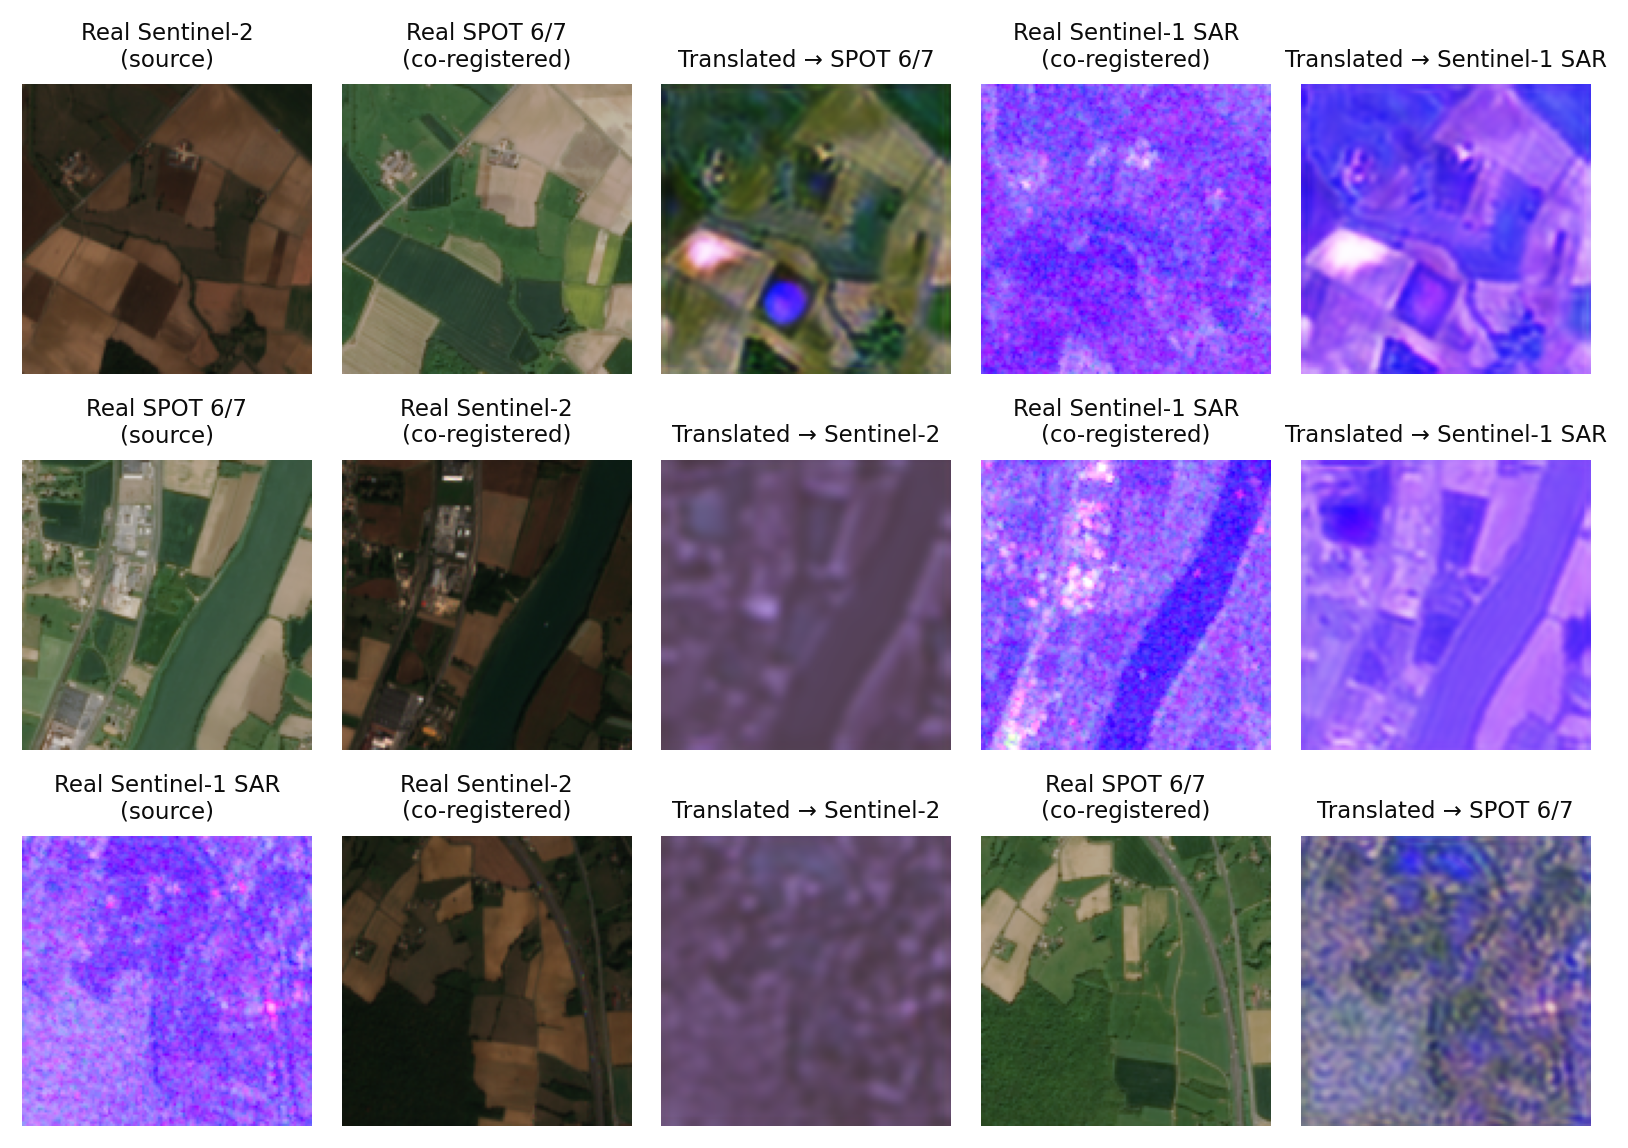
\includegraphics[width=0.7\textwidth]{figures/fig_paired_translation.png}
\caption{Translations of one held-out patch per source domain (first column of each row) into the two other domains, next to the real co-registered patch of each target domain. The style is the centroid embedding of the target domain, and the patches were chosen by a fixed random seed before inspection. Sentinel-1 patches are displayed as VV, VH, and the saturated difference channel in red, green, and blue.}
\label{fig:paired}
\end{figure*}

\begin{table}[t]
\centering
\caption{Translation into each target on held-out patches. PSNR (dB) against the co-registered real target patch for the translation, for the copied source (Copy) and for a constant target-mean image (Const.); Style is the share of outputs that the encoder assigns to the target domain; Edge is the edge-map correlation with the source.}
\label{tab:gen}
\footnotesize
\setlength{\tabcolsep}{3.5pt}
\begin{tabular}{@{}lccccc@{}}
\toprule
\textbf{Pair} & \textbf{Transl.} & \textbf{Copy} & \textbf{Const.} & \textbf{Style} & \textbf{Edge} \\
\midrule
S2 $\rightarrow$ SPOT   & 14.6 & 13.1 & 17.2 & 57\% & 0.82 \\
S2 $\rightarrow$ SAR    & 14.6 & 5.7 & 20.5 & 18\% & 0.87 \\
SPOT $\rightarrow$ S2   & 13.5 & 13.1 & 17.8 & 29\% & 0.71 \\
SPOT $\rightarrow$ SAR  & 16.8 & 7.4 & 20.5 & 80\% & 0.82 \\
SAR $\rightarrow$ S2    & 13.3 & 5.7 & 17.8 & 12\% & 0.94 \\
SAR $\rightarrow$ SPOT  & 13.0 & 7.4 & 17.2 & 45\% & 0.92 \\
\bottomrule
\end{tabular}
\end{table}

The style vector is used: the PSNR for the source to translation is higher than for the source to the real target domain (by 3.3 to 7.6~dB) for 5 of 6 pairs, and parcels are still recognizable in the figure, even though the road is not. The target radiometry is not reproduced: the constant image is correlated better with the real target patch than the translation for all 6 pairs (by 2.6 to 5.9~dB; the correlation is always higher than 0.61, better for pairs involving SAR than for others), the encoder assigns the outputs to the target domain in only 12\% to 80\% of the cases, and translations into Sentinel-2 are a blurred purple-gray haze whose channel means are equal within 0.001 for all 3 sources, and much brighter than real Sentinel-2 patches (by The identity mapping of Sentinel-2 is also not very well reproduced (13.7~dB, while for SPOT and SAR 20.3~dB and 24.3~dB, respectively); Sentinel-2 is the least strong of the generator both as source and as target. The different modalities acquired at different times constrained the degree to which the pixels may be matched, but did not account for the poorer transmission of a constant image.

The style space of the two points was sampled by interpolating between the two domain centroids, $z(\alpha)=(1-\alpha)\bar z_a+\alpha\bar z_b$ with the points renormalized to unit length, for 300 sets of source patches. The two pairs involving SAR resulted in a smooth change in output, close to linear (linearity ratio 0.91 and 0.96, monotone for 96\% and 100\% of the patches, respectively). The change is 10\% smaller for Sentinel-2 and SPOT, and only the first step ($0<\alpha<0.25$) contains the majority of the change 89\% of the patches, with only 41\% of them being monotone. There are 1.59~M parameters for the generator and 0.89~M for the encoder, and the CPU takes approximately 84~ms for a translation per patch.

Fig.~\ref{fig:interp} shows this interpolation for one held-out SPOT~6/7 source patch.

\begin{figure}[t]
\centering
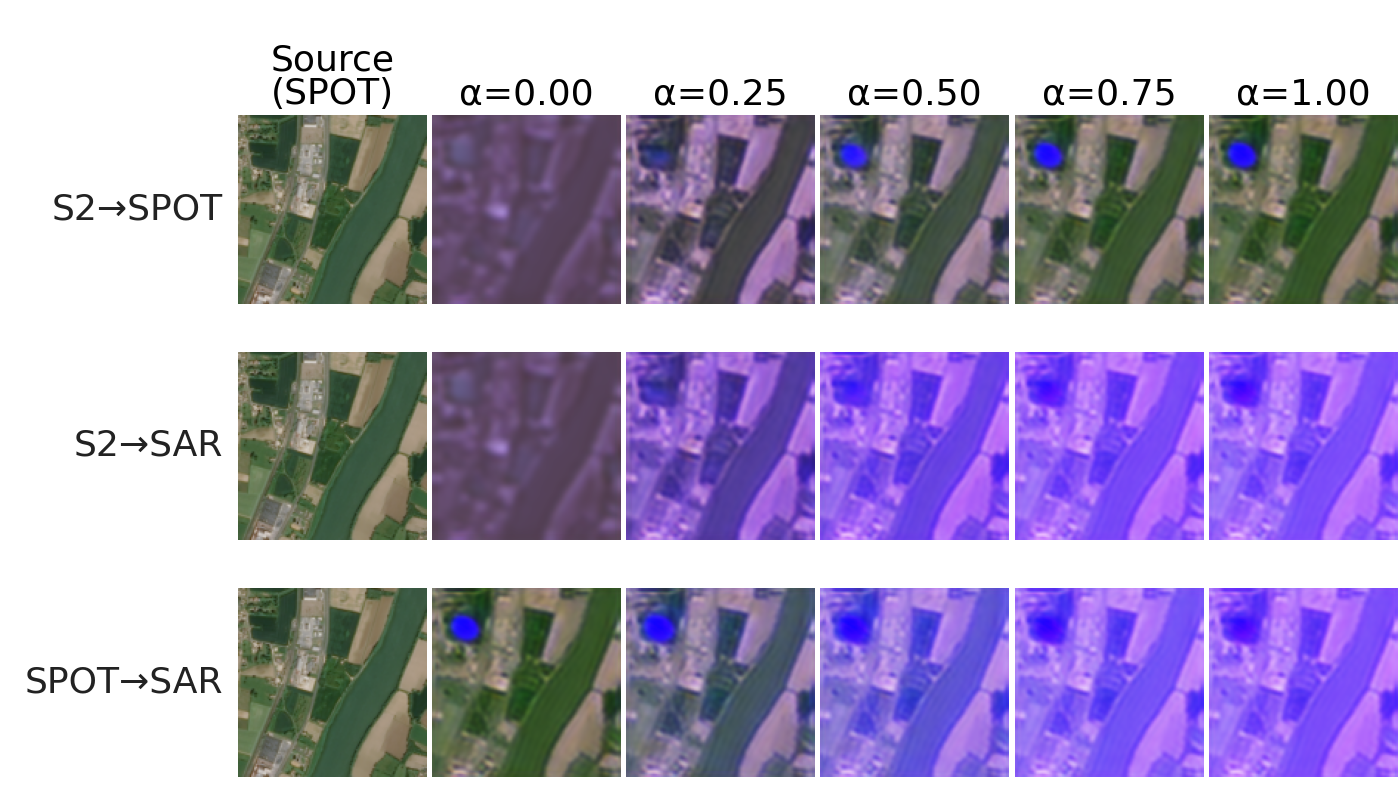
\includegraphics[width=\columnwidth]{figures/fig_interp_compact.png}
\caption{Interpolation of the style vector between two domain centroids, $z(\alpha)=(1-\alpha)\bar z_a+\alpha\bar z_b$ renormalized to unit length, applied to one held-out SPOT~6/7 source patch (first column). Each row is a pair of domains $a \rightarrow b$ and $\alpha$ runs from the style of $a$ ($\alpha=0$) to the style of $b$ ($\alpha=1$). The patch was chosen by a fixed random seed before inspection.}
\label{fig:interp}
\end{figure}

The architectural objectives of Table~\ref{tab:gap} are achieved: there is no labeling of the domain, a single generator for all the ordered pairs of three domains, and a continuous 64-dimensional domain code. None of the cited methods were trained on the same data as used for this work, and the numbers published for these methods are from other data and tasks, so any comparison to the quality of the result is not warranted, and no claim is made that the approach is better than SS(DA)$^2$, StarGAN~v2, or any of the other methods.

\section{Limitations}
\label{sec:limitations}
The above results have some restrictions. First, the held-out patches are from one Sentinel-2 tile, and the training set is largely from two other tiles, and so the results are a blend of model quality and a shift towards a different region; domain centroids are from different regions to the patches they're applied to. Second, there is no simultaneous modality, limiting the ability to agree at the pixel level with the co-registered reference, and there are artifacts in the preprocessing (saturated SAR channel and synthetic fourth SPOT channel). Third, for each model, the training was performed only once on a CPU with only 12 epochs of the generator and 10 epochs of the encoder (Sec.~\ref{sec:setup}), and the training loops were not seeded, no run-to-run variation was tested, no ablation of the six generator losses was performed, and no other method of translation was trained on the same data. Fourth, PSNR and SSIM are used for the degree of agreement with a co-registered image, not for realism, and the rate of style transfer is evaluated by the same encoder used for conditioning the generator. Fifth, only three sensor domains, one geographic setting and 1,500 of 2,433 locations were utilized; the larger MSC-France corpus that was foreseen forencoder pretraining and the angle-conditioning were not used. Finally, generalisation of unseen sensor pairs and downstream accuracy are not assessed.

\section{Conclusion and Future Work}
The proposed framework was a novel multi-domain self-supervised adaptation framework for satellite-based image data, which consisted of two main components: a contrastive domain encoder for learning label-free, continuous embeddings of the sensor style of the images, and an AdaIN-conditioned generator for generating an image in an arbitrary target style, given a source patch and its learned embedding from the domain encoder. The framework has the potential to comply with the design goals at the architectural level: No domain labels, one model for all ordered domain pairs, a continuous domain code, trained on real PASTIS-HD imagery (Sentinel-2, SPOT~6/7, Sentinel-1 SAR). There is a limited measured quality: the encoder identifies the sensor moderately (65.8\% vs 33.3\% chance) and the generator preserves the structure of the scene and uses the style vector, but cannot reproduce the radiometry of the measured sensor; translations into Sentinel-2 do not work.

Future work will involve (i) replacing the augmented-view positives with sensor-aware positive pairs based on spatial and temporal proximity and pretraining on a larger corpus MSC-France; (ii) fixing data issues found here, including all PASTIS-HD patches, a tile-stratified split and temporally matched acquisitions, a non-saturating SAR channel; (iii) training wider networks longer on a GPU with seeded runs, loss ablations and same-data baselines; and (iv) testing leave-one-domain-pair-out and zero-shot (SpaceNet~6) generalization and downstream crop classification and segmentation.

\bibliographystyle{IEEEtran}
\bibliography{references}

\end{document}
"
% Camera-ready build (authors shown): pdflatex main.tex
\ifdefined\ANON
\author{
\IEEEauthorblockN{Anonymous Authors}
\IEEEauthorblockA{Anonymous Affiliation}
}
\else
\author{
\IEEEauthorblockN{Shivangi\textsuperscript{1}, Benedict Tephila M.\textsuperscript{2}, Naveen J.\textsuperscript{3}}
\IEEEauthorblockA{
Department of Computer Science and Engineering \\
CHRIST (Deemed to be University), Bangalore -- 560029, India \\
\textsuperscript{1}shivangi.a@mtech.christuniversity.in,
\textsuperscript{2}benedict.tephila@christuniversity.in,
\textsuperscript{3}naveen.j@christuniversity.in}
}
\fi

\maketitle

\begin{abstract}
The performance of deep learning models trained for the analysis of satellite images suffers when the same land-cover classes are captured by a different sensor, at a different season, or in a different region. Current domain-adaptation techniques typically require labeled target data, a fixed domain library, or both, but these are hard to obtain with evolving and expanding multi-sensor archives. Firstly, we present a continuous domain encoder that produces a label-free style embedding from unlabeled multi-sensor patches through the use of a contrastive (InfoNCE) pretext task, and secondly, we introduce a unified conditional generator that creates a style conditioned transformation of the content of the source patch into an arbitrary style of the target domain by learning a style embedding as a continuous latent space rather than a discrete class label. Both networks trained on 1,200 patches per sensor provided by PASTIS-HD (Sentinel-2, SPOT~6/7, Sentinel-1 SAR) and tested on 300 held-out patches per sensor from a region that is mostly different. The encoder successfully completes its pretext task, but recognises the sensor with only some success (65.8\% as opposed to 33.3\% chance). The generator maintains the scene structure and performs well on the pairs that contain SAR, but does not reproduce the radiometry of the target sensor: a constant image is closer to the actual target patch than a translation, and translated images end up as a source-independent color cast, when SAR is present in one of the pairs. This paper does not include generalization to unseen sensor pairs, nor does it include downstream accuracy.
\end{abstract}

\begin{IEEEkeywords}
domain adaptation, self-supervised learning, generative adversarial networks, contrastive learning, multi-sensor satellite imagery, image-to-image translation
\end{IEEEkeywords}

\section{Introduction}

Satellite remote sensing has now evolved from one single mission to a constellation of optical and radar satellites, seeing the Earth's surface together and in succession, such as Sentinel-2, Landsat, SPOT and a growing number of commercial very-high-resolution (VHR) and synthetic aperture radar (SAR) satellites. The use of deep learning models for land-cover classification, crop mapping and change detection has been increasingly placed on the ability to perform on this multi-sensor heterogeneous archive, as opposed to the single sensor they were trained on.

It is hard to achieve this cross-sensor requirement in practice. These include different radiometric calibration, spectral response, spatial resolution, and noise properties for each sensor, which vary from atmospheric haze and calibration drift in optical imagery to speckle noise and incidence-angle-dependent backscatter in SAR. Consequently, a model trained with the statistics from one sensor may exhibit a dramatic decrease in accuracy when applied to another sensor, even when the land-cover classes are the same. Modeling often requires the adaptation to a new domain with little or no target domain labeled data because of the high cost of acquiring and annotating imagery from all sensors of interest.

The current methods can be classified into two families. Satellite-specific methods, like multi-source standardization~\cite{tasar2020standardgan} normalize translation on a discrete domain identity that is manually assigned to each satellite and are claimed to have difficulty with unseen combinations of domains. However, self-supervised methods like SS(DA)$^2$~\cite{zhang2023ssdada} do not require labels or an explicit domain boundary and only translate between two satellites at a time, meaning that a new method must be developed for each new pair of satellites. In the general image-translation literature, StarGAN~\cite{choi2018stargan} and StarGAN~v2~\cite{choi2020starganv2} integrate a multitude of domains into a single generator, with StarGAN~v2 additionally using a continuous style code, and performing regular evaluations on natural images. Diffusion-based translators~\cite{vinholi2024multisensor,kieu2025universal} are more faithful but work on discrete domain sets, with higher inference cost.

The combination of label-free training, a continuous (discretely labeled is not the only option) representation of the domain and a single generator that can translate into an arbitrary target style is not yet explicitly provided in the literature for satellite images. It is the motivation for the present work to fill this gap.

The first two properties are addressed by further developing the pairwise approach of the SS(DA)$^2$ paradigm to a continuous, StarGAN~v2-style unified generator without the need for any domain-specific conditioning: A domain encoder produces a uniform embedding of the domain characteristics of each patch, and a single generator, modulated by the embedding through the use of AdaIN, maps a source patch to the domain of any target patch's embedding. These two components are designed, implemented, and evaluated using held-out data, which is not covered by this paper.

This paper makes the following contributions:
\begin{itemize}
\item A self-supervised contrastive domain encoder to generate label-free, continuous embeddings of sensor/style features from unlabeled multi-sensor patches.
A single AdaIN-modulated conditional generator conditioned on this embedding, instead of a discrete domain code, so no retraining per domain pair is required for the translation to an arbitrary target style.
An objective for six terms of training that maintains the geospatial content while changing the style of the content.
\item held out evaluation on real PASTIS-HD data that reports what works (label-free continuous embeddings, structure preserving, style conditioned translation) and what doesn't (moderate sensor information in the embedding, target radiometry not reproduced).
\end{itemize}

\section{Related Work}

\subsection{Domain Adaptation for Satellite Imagery}
StandardGAN~\cite{tasar2020standardgan} is used to standardize each source domain towards a common reference for semantic segmentation of multi-source VHR satellite images towards the common reference. It works on a set of discrete and enumerated domains, and according to the report of its authors, it has trouble maintaining the content of the images and it has poor generalisation ability with respect to sensor combinations not encountered at the time of standardisation. SS(DA)$^2$~\cite{zhang2023ssdada} does not require labeled target data or the domain boundary: a contrastive, domain-agnostic GAN translates between two satellite domains with unlabeled images. The downside to this, and what is being solved here, is that it is pairwise: each model can accommodate only two satellites.

\subsection{Multi-Domain Image-to-Image Translation}
StarGAN~\cite{choi2018stargan} combined multi-domain translation into a single generator, and used a discrete one-hot domain vector as the condition. It is replaced in StarGAN~v2~\cite{choi2020starganv2} by a continuous style code from a mapping network or style encoder fed into AdaIN~\cite{huang2017adain} and it is evaluated on natural image datasets, using realism metrics (e.g., FID), and not on satellite imagery. Multi-sensor optical image translation~\cite{vinholi2024multisensor} and universal multi-domain routing~\cite{kieu2025universal} are both based on diffusion and enhance fidelity, but the router still chooses from a discrete set of domain experts and iterative sampling is more expensive than one feed-forward GAN pass, especially for large mosaics of satellites.

\section{Research Gap and Motivation}
The most similar methods are compared to the properties targeted here in Table~\ref{tab:gap}. SS(DA)$^2$ is label-free and pairwise while StarGAN~v2 is continuous domain representation and supervised discrete domain identity at training time, and designed for remote sensing; StandardGAN is designed for satellite imagery and requires discrete domain identity. All the methods reviewed here did not accept labels and used a continuous domain without a generator specifically designed for and tested on satellite images. This project's goals, ~1 and ~2, are specifically aimed at this combination: Continuous domain encoder without labels, and a single generator conditioned on its embedding.

\begin{table}[t]
\centering
\caption{Qualitative comparison of properties relevant to the identified research gap.}
\label{tab:gap}
\resizebox{\linewidth}{!}{%
\begin{tabular}{@{}lccc@{}}
\toprule
\textbf{Method} & \textbf{Label-free} & \textbf{Continuous domain repr.} & \textbf{Satellite-specific} \\
\midrule
StandardGAN~\cite{tasar2020standardgan}    & \ding{55} & \ding{55} & \ding{51} \\
SS(DA)$^2$~\cite{zhang2023ssdada}          & \ding{51} & \ding{55} (pairwise) & \ding{51} \\
StarGAN~\cite{choi2018stargan}             & \ding{55} & \ding{55} & \ding{55} \\
StarGAN~v2~\cite{choi2020starganv2}        & \ding{55} & \ding{51} & \ding{55} \\
\textbf{Proposed (Objectives 1--2)}        & \ding{51} & \ding{51} & \ding{51} \\
\bottomrule
\end{tabular}}
\end{table}

\section{Proposed Methodology}

\begin{figure*}[t]
\centering
\resizebox{\textwidth}{!}{%
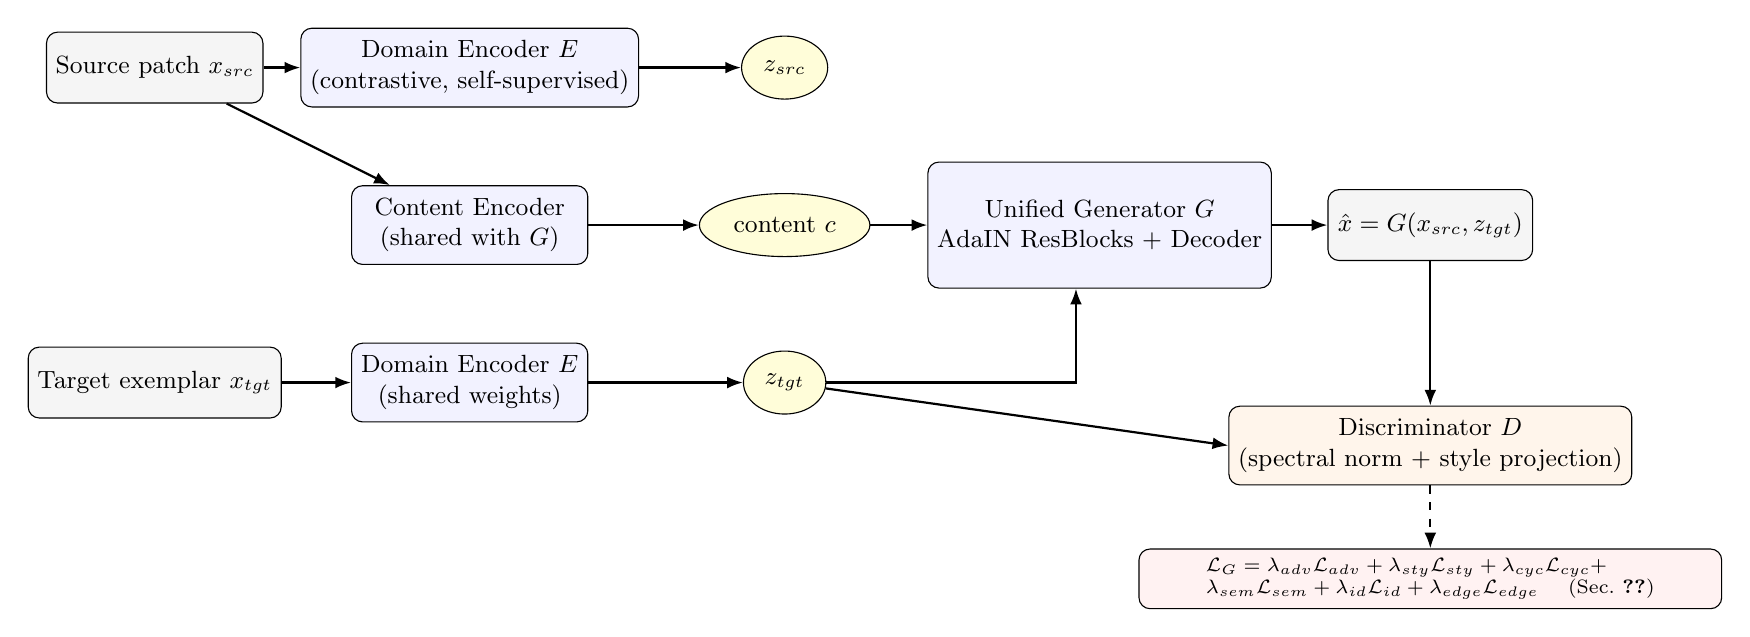
\begin{tikzpicture}[
  node distance=8mm and 10mm,
  box/.style={draw, rounded corners, align=center, minimum height=1.0cm, font=\small, fill=blue!5},
  data/.style={draw, rounded corners, align=center, minimum height=0.9cm, font=\small, fill=gray!8},
  vec/.style={draw, ellipse, align=center, minimum height=0.8cm, font=\small, fill=yellow!15},
  lossbox/.style={draw, rounded corners, align=left, font=\scriptsize, fill=red!5},
  arr/.style={-{Latex[length=2mm]}, thick}
]
  \node[data]                              (xsrc) at (0,6)    {Source patch $x_{src}$};
  \node[data]                              (xtgt) at (0,2)    {Target exemplar $x_{tgt}$};

  \node[box, minimum width=3.0cm]          (E1)   at (4.0,6)  {Domain Encoder $E$\\(contrastive, self-supervised)};
  \node[box, minimum width=3.0cm]          (CE)   at (4.0,4)  {Content Encoder\\(shared with $G$)};
  \node[box, minimum width=3.0cm]          (E2)   at (4.0,2)  {Domain Encoder $E$\\(shared weights)};

  \node[vec]                               (zsrc) at (8.0,6)  {$z_{src}$};
  \node[vec]                               (c)    at (8.0,4)  {content $c$};
  \node[vec]                               (ztgt) at (8.0,2)  {$z_{tgt}$};

  \node[box, minimum width=3.2cm, minimum height=1.6cm] (G) at (12.0,4) {Unified Generator $G$\\AdaIN ResBlocks + Decoder};

  \node[data, minimum width=2.6cm]         (xfake) at (16.2,4) {$\hat{x} = G(x_{src}, z_{tgt})$};

  \node[box, fill=orange!8, minimum width=3.0cm] (D) at (16.2,1.2) {Discriminator $D$\\(spectral norm + style projection)};

  \draw[arr] (xsrc) -- (E1);
  \draw[arr] (xsrc) -- (CE);
  \draw[arr] (xtgt) -- (E2);
  \draw[arr] (E1) -- (zsrc);
  \draw[arr] (CE) -- (c);
  \draw[arr] (E2) -- (ztgt);
  \draw[arr] (c) -- (G);
  \draw[arr] (ztgt.east) -| ([xshift=-3mm]G.south);
  \draw[arr] (G) -- (xfake);
  \draw[arr] (xfake) -- (D);
  \draw[arr] (ztgt) -- (D.west);

  \node[lossbox, below=8mm of D, minimum width=7.4cm] (losses) {
    $\mathcal{L}_G = \lambda_{adv}\mathcal{L}_{adv} + \lambda_{sty}\mathcal{L}_{sty} + \lambda_{cyc}\mathcal{L}_{cyc} +$\\
    $\lambda_{sem}\mathcal{L}_{sem} + \lambda_{id}\mathcal{L}_{id} + \lambda_{edge}\mathcal{L}_{edge}$ \quad (Sec.~\ref{sec:objective})
  };
  \draw[arr, dashed] (D.south) -- (losses.north);
\end{tikzpicture}}
\caption{Simplified architecture of the two components reported here: the self-supervised domain encoder $E$ (Sec.~\ref{sec:encoder}) and the AdaIN-conditioned generator $G$ with projection discriminator $D$ (Sec.~\ref{sec:generator}). The source embedding $z_{src}$ is reused in two further passes through $G$, omitted for clarity, for the cycle and identity losses of Sec.~\ref{sec:objective}.}
\label{fig:architecture}
\end{figure*}

The two components that are addressed in this paper are shown in Fig.~\ref{fig:architecture}. A domain encoder $E$ is used to project an unlabeled image patch to a continuous style embedding, a content encoder $G$ is used as the downsampling path of the generator to extract a domain-invariant spatial content code, and a unified generator $G$ is used to combine the content of a source patch with the embedding of a target patch to generate a translation, which is then evaluated by a projection discriminator $D$.

\subsection{Self-Supervised Continuous Domain Encoder}
\label{sec:encoder}
This is achieved by the encoder $E_\theta$ which maps an $H \times W$ patch containing $C$ channels (4 in this implementation, corresponding to 3 optical channels and 1 auxiliary channel, see Sec.~\ref{sec:dataset}) to a continuous embedding $z \in \mathbb{R}^{64}$. The network is composed of an input-adapter convolution, followed by three stride-2 convolutional blocks (Conv--InstanceNorm--LeakyReLU) to gradually reduce the spatial resolution, but expand the channel width, followed by a squeeze-and-excitation (SE) block~\cite{hu2018senet} which recalibrates the responses channel-wise.

Instead of pooling to a class score, the encoder calculates two types of statistics, the first-order mean $\mu$ and the second-order standard deviation $\sigma$ of the final feature map, representing the radiometric and textural style of the patch, respectively, without relying on spatial content:
\begin{equation}
\mu_c = \frac{1}{HW}\sum_{i,j} h_{c,i,j}, \qquad
\sigma_c = \sqrt{\frac{1}{HW}\sum_{i,j}(h_{c,i,j}-\mu_c)^2 + \epsilon}
\label{eq:stats}
\end{equation}
where $h$ is the feature map after the SE block. The concatenated statistics $[\mu;\sigma]$ (optionally fused with a projected acquisition-angle feature when angle metadata is available, unused in the sensor-only experiment reported here) are passed through a multilayer perceptron projection head and L2-normalized onto the unit hypersphere:
\begin{equation}
z = \frac{f_\phi([\mu;\sigma])}{\lVert f_\phi([\mu;\sigma]) \rVert_2}, \qquad z \in \mathbb{R}^{64}.
\label{eq:embed}
\end{equation}

The encoder is pretrained with no domain labels using a contrastive pretext task in the style of InfoNCE~\cite{oord2018cpc}. Two independently augmented views ($z_1, z_2$) of the same patch (random flips and 90\textdegree{} rotations) are treated as a positive pair, and all other patches in the training batch act as negatives:
\begin{equation}
\mathcal{L}_{con} = -\frac{1}{2B}\sum_{i=1}^{B}\Big[
\log\frac{e^{\,z_{1,i}\cdot z_{2,i}/\tau}}{\sum_{j} e^{\,z_{1,i}\cdot z_{2,j}/\tau}}
+
\log\frac{e^{\,z_{2,i}\cdot z_{1,i}/\tau}}{\sum_{j} e^{\,z_{2,i}\cdot z_{1,j}/\tau}}
\Big]
\label{eq:infonce}
\end{equation}
where $B$ is the batch size and $\tau$ is a temperature hyperparameter. Because positives and negatives come from augmentation rather than sensor labels, no supervision of domain identity is used, and any patch can be projected into the same continuous space at inference time.

\subsection{Unified Conditional Generator}
\label{sec:generator}
The generator $G_\psi$ takes a source patch $x_{src}$ and a target embedding $z_{tgt}$ (produced by the frozen encoder $E$ on a target-domain exemplar) and synthesizes a translated patch $\hat{x} = G_\psi(x_{src}, z_{tgt})$. A single generator instance is shared across all domains: the target style is entirely determined by $z_{tgt}$, so translation into any domain the encoder can embed -- rather than only domains enumerated at training time -- requires no architectural change or additional parameters.

The content path follows an encoder-bottleneck-decoder design in the spirit of StarGAN~v2~\cite{choi2020starganv2}, adapted to be label-free. A content encoder with reflection-padded convolutions and instance normalization downsamples $x_{src}$ to a domain-invariant content code $c = \mathrm{Enc}_c(x_{src})$. This code is passed through four residual blocks modulated by Adaptive Instance Normalization (AdaIN)~\cite{huang2017adain}, which injects the target style at every block:
\begin{equation}
\mathrm{AdaIN}(h, z) = \gamma(z)\cdot\frac{h - \mu(h)}{\sigma(h)} + \beta(z)
\label{eq:adain}
\end{equation}
where $\mu(h), \sigma(h)$ are the per-channel instance statistics of the intermediate feature map $h$, and $\gamma(z) = W_\gamma z + b_\gamma$, $\beta(z) = W_\beta z + b_\beta$ are affine parameters regressed from the continuous embedding. The decoder mirrors the encoder with two AdaIN-modulated upsampling stages; bilinear (rather than nearest-neighbor or transposed-convolution) upsampling is used to avoid checkerboard artifacts, followed by a reflection-padded output convolution with a $\tanh$ activation.

\subsection{Discriminator with Continuous Style Projection}
The discriminator $D_\xi$ is a multi-scale PatchGAN with spectral normalization~\cite{miyato2018spectral} applied to every convolutional layer, which stabilizes adversarial training by bounding the Lipschitz constant of each layer. In addition to an unconditional real/fake head, $D_\xi$ projects its intermediate features onto the conditioning embedding $z$:
\begin{equation}
D_\xi(x, z) = D_{uncond}(x) + \frac{\langle \phi(x), W_{proj}\,z\rangle}{\sqrt{d}}
\label{eq:disc}
\end{equation}
where $\phi(x)$ is the discriminator's penultimate feature map, $W_{proj}$ is a learned linear projection of the embedding, and $d$ is the feature dimension. This term penalizes translations whose visual style does not match the conditioning embedding $z$, complementing the encoder's own style-reconstruction signal (Sec.~\ref{sec:objective}).

\subsection{Composite Training Objective}
\label{sec:objective}
The generator is trained with a weighted sum of six loss terms, each targeting a specific failure mode observed in unconstrained multi-domain translation:

\emph{Adversarial loss} (least-squares GAN~\cite{mao2017lsgan}), encouraging $\hat{x}$ to be indistinguishable from real target-domain patches under the style-conditioned discriminator:
\begin{align}
\mathcal{L}_D &= \tfrac{1}{2}\mathbb{E}\big[(D_\xi(x_{tgt}, z_{tgt}) - 1)^2\big] + \tfrac{1}{2}\mathbb{E}\big[D_\xi(\hat{x}, z_{tgt})^2\big] \\
\mathcal{L}_{adv} &= \mathbb{E}\big[(D_\xi(\hat{x}, z_{tgt}) - 1)^2\big]
\label{eq:adv}
\end{align}

\emph{Style-reconstruction loss}, requiring the target style to be measurable in the output by re-encoding it:
\begin{equation}
\mathcal{L}_{sty} = \mathbb{E}\,\lVert E(\hat{x}) - z_{tgt} \rVert_1
\label{eq:sty}
\end{equation}

\emph{Cycle-consistency loss}~\cite{zhu2017cyclegan}, translating $\hat{x}$ back toward the source style and requiring recovery of the original patch, which discourages mode collapse across domains:
\begin{equation}
\mathcal{L}_{cyc} = \mathbb{E}\,\lVert G(\hat{x}, z_{src}) - x_{src} \rVert_1
\label{eq:cyc}
\end{equation}

\emph{Semantic-preservation loss}, penalizing drift in the domain-invariant content code between the source and the translation, so that geospatial layout (parcel boundaries, roads) is not altered by the style change:
\begin{equation}
\mathcal{L}_{sem} = \mathbb{E}\,\lVert \mathrm{Enc}_c(\hat{x}) - \mathrm{Enc}_c(x_{src}) \rVert_1
\label{eq:sem}
\end{equation}

\emph{Identity loss}, requiring that conditioning the generator on the source's own style leaves the patch unchanged:
\begin{equation}
\mathcal{L}_{id} = \mathbb{E}\,\lVert G(x_{src}, z_{src}) - x_{src} \rVert_1
\label{eq:id}
\end{equation}

\emph{Edge-preservation loss}, comparing Sobel gradient magnitudes between $\hat{x}$ and $x_{src}$ to keep agricultural parcel boundaries and road edges sharp:
\begin{equation}
\mathcal{L}_{edge} = \mathbb{E}\,\lVert \nabla_{Sobel}(\hat{x}) - \nabla_{Sobel}(x_{src}) \rVert_1
\label{eq:edge}
\end{equation}

The total generator objective is
\begin{align}
\mathcal{L}_G ={}& \lambda_{adv}\mathcal{L}_{adv} + \lambda_{sty}\mathcal{L}_{sty} + \lambda_{cyc}\mathcal{L}_{cyc} \notag \\
& + \lambda_{sem}\mathcal{L}_{sem} + \lambda_{id}\mathcal{L}_{id} + \lambda_{edge}\mathcal{L}_{edge}
\label{eq:total}
\end{align}
with weights listed in Table~\ref{tab:hyperparams}. The framework additionally defines a geometric (SSIM-style) preservation loss $\mathcal{L}_{geo}$, activated when either the source or target domain is an off-nadir viewing-angle domain; because the PASTIS-HD experiment reported in Sec.~\ref{sec:results} uses only sensor domains, $\mathcal{L}_{geo}$ is inactive ($\lambda_{geo}\mathcal{L}_{geo}=0$) for the results shown here.

\section{Dataset and Preprocessing}
\label{sec:dataset}
Experiments are conducted on patches that are taken from PASTIS-HD~\cite{garnot2021panoptic,astruc2024omnisat} a public benchmark of $2{,}433$ co-registered agricultural-parcel locations in France for which SAR time series from Sentinel-2 and Sentinel-1 datasets are provided, and in the HD extension a very-high-resolution image from SPOT~6/7. A conversion pipeline matches up patches by identifier and exports a $128\times128$ 4-channel tensor per modality, per location: Sentinel-2 Red, Green, Blue and near-infrared channels are kept as is; SPOT~6/7 is resized from $1280\times1280$ and provided with a synthetic near-infrared proxy channel, and the two polarizations of Sentinel-1 (VV and VH) are extended with a derived ratio and average channel, and are converted from decibel to linear units. All modalities have the range of [-1,1]. In this experiment, the first $1{,}500$ locations per domain in identifier order (the patch cap of the pipeline) is converted from three Sentinel-2 tiles. In this case, 80\% of the patches are used as training data and 20\% are held out, with 1200 used in the training set and 300 held out, meaning that all held out patches are in a single region, only slightly underrepresented in training, and the evaluation is largely on a different region. The modalities are co-registered, but not simultaneous: the first Sentinel-1 acquisition is 11 days after the first Sentinel-2 acquisition (median) and the SPOT imagery is provided from 2019. After conversion, the SAR difference channel is saturated at $+1$ for 97.9\% of its values. Random flips, rotations by 90\textdegree{} and small Gaussian radiometric noise $\sigma \sim \mathcal{U}[0, 0.01]$ are added to the training patches.

\section{Experimental Setup}
\label{sec:setup}
It is implemented in Python~3.13 with PyTorch~$\geq$2.4 and is controlled by a single command line entry point, which first trains the domain-encoder, then trains the generator and discriminator jointly. All training and evaluation were performed on the CPU of a laptop with following specification: Intel Core i7-9750H, 6 core, 7.8~GB RAM. The width of the generator and discriminator (base width 32) is kept narrow to ensure this compute is tractable for training, rather than be close to a reported baseline. For the results in Sec.~\ref{sec:results} the following hyperparameters were used, as shown in Tab.~\ref{tab:hyperparams}.

\begin{table}[t]
\centering
\caption{Training hyperparameters.}
\label{tab:hyperparams}
\begin{tabular}{@{}ll@{}}
\toprule
\textbf{Stage 1 -- Domain Encoder} & \textbf{Value} \\
\midrule
Embedding dimension $d$            & 64 \\
Optimizer                          & AdamW \\
Learning rate                      & $5\times10^{-4}$ \\
Weight decay                       & $1\times10^{-4}$ \\
Contrastive temperature $\tau$     & 0.07 \\
Epochs                             & 10 \\
\midrule
\textbf{Stage 2 -- Generator / Discriminator} & \textbf{Value} \\
\midrule
Base channel width                 & 32 \\
Residual blocks                    & 4 \\
Optimizer ($G$, $D$)               & Adam ($\beta_1{=}0.5$, $\beta_2{=}0.999$) \\
Learning rate ($G$, $D$)           & $3\times10^{-4}$ \\
LR schedule                        & Cosine annealing, $\eta_{min}{=}10^{-5}$ \\
Gradient clipping (max norm)       & 1.0 \\
Epochs                             & 12 \\
Batch size                         & 8 \\
$\lambda_{adv},\lambda_{sty},\lambda_{id}$ & 1.0 each \\
$\lambda_{sem}$, $\lambda_{edge}$  & 2.0 each \\
$\lambda_{cyc}$                    & 10.0 \\
\bottomrule
\end{tabular}
\end{table}

\section{Results and Discussion}
\label{sec:results}
All results are on the 300 withheld patches per domain with a constant protocol and are only a single measurement from one trained model. Target domains are L2-normalized mean of the embedding of 1200 patches in the target domain, which are the \emph{centroid} of the domain (the training patches are used in the embedding process, but not for the evaluation step). The images are rescaled to $[0,1]$ against the co-registered real target patch, having two reference baselines: ``Copy'' for the untranslated source patch, and ``Const.'' for the constant image that corresponds to the mean of the target domain.

\subsection{Domain encoder (Objective~1)}
Table~\ref{tab:enc} summarizes the encoder. It achieves a solution to its contrastive task on held-out patches (loss 0.24 compared to 2.08 with an uninformative embedding; 88.2\% top-1 retrieval of the second view on 900 patches), while its embeddings are uniformly distributed over the hypersphere rather than in three concentrated clusters. They describe the sensor moderately: 65.8\% of held out patches are correctly assigned to the sensor by the nearest centroid as compared with 33.3\% randomly; the sensors overlap (silhouette coefficient 0.11); effective dimensionality is about 4. The co-registered patch of another sensor is retrieved at chance level, which means that the embedding does not contain information about the scene that is shared across sensors. One possible reason (not tested) is that instance discrimination does not include a term to group the patches of one sensor, and that proximity-based positive pairs as planned in the project plan were not used.

\begin{table}[t]
\centering
\caption{Domain encoder on 300 held-out patches per domain (S2: Sentinel-2).}
\label{tab:enc}
\begin{tabular}{@{}lc@{}}
\toprule
\textbf{Measurement} & \textbf{Result} \\
\midrule
Held-out InfoNCE loss (batch 8; chance 2.08)        & 0.24 \\
Top-1 instance retrieval among 900 patches          & 88.2\% \\
Nearest-centroid domain accuracy (chance 33.3\%)    & 65.8\% \\
\quad recall S2 / SPOT / SAR                        & 62.7 / 74.3 / 60.3\% \\
5-nearest-neighbor domain accuracy                  & 63.7\% \\
Cosine similarity within / between domains          & 0.32 / 0.04 \\
Silhouette coefficient (cosine distance)            & 0.11 \\
Participation ratio (of 64 dimensions)              & 3.85 \\
Same-location retrieval across sensors, top-1       & 0.3\% (chance 0.3\%) \\
\bottomrule
\end{tabular}
\end{table}

\subsection{Conditional generator (Objective~2)}
\begin{figure*}[t]
\centering
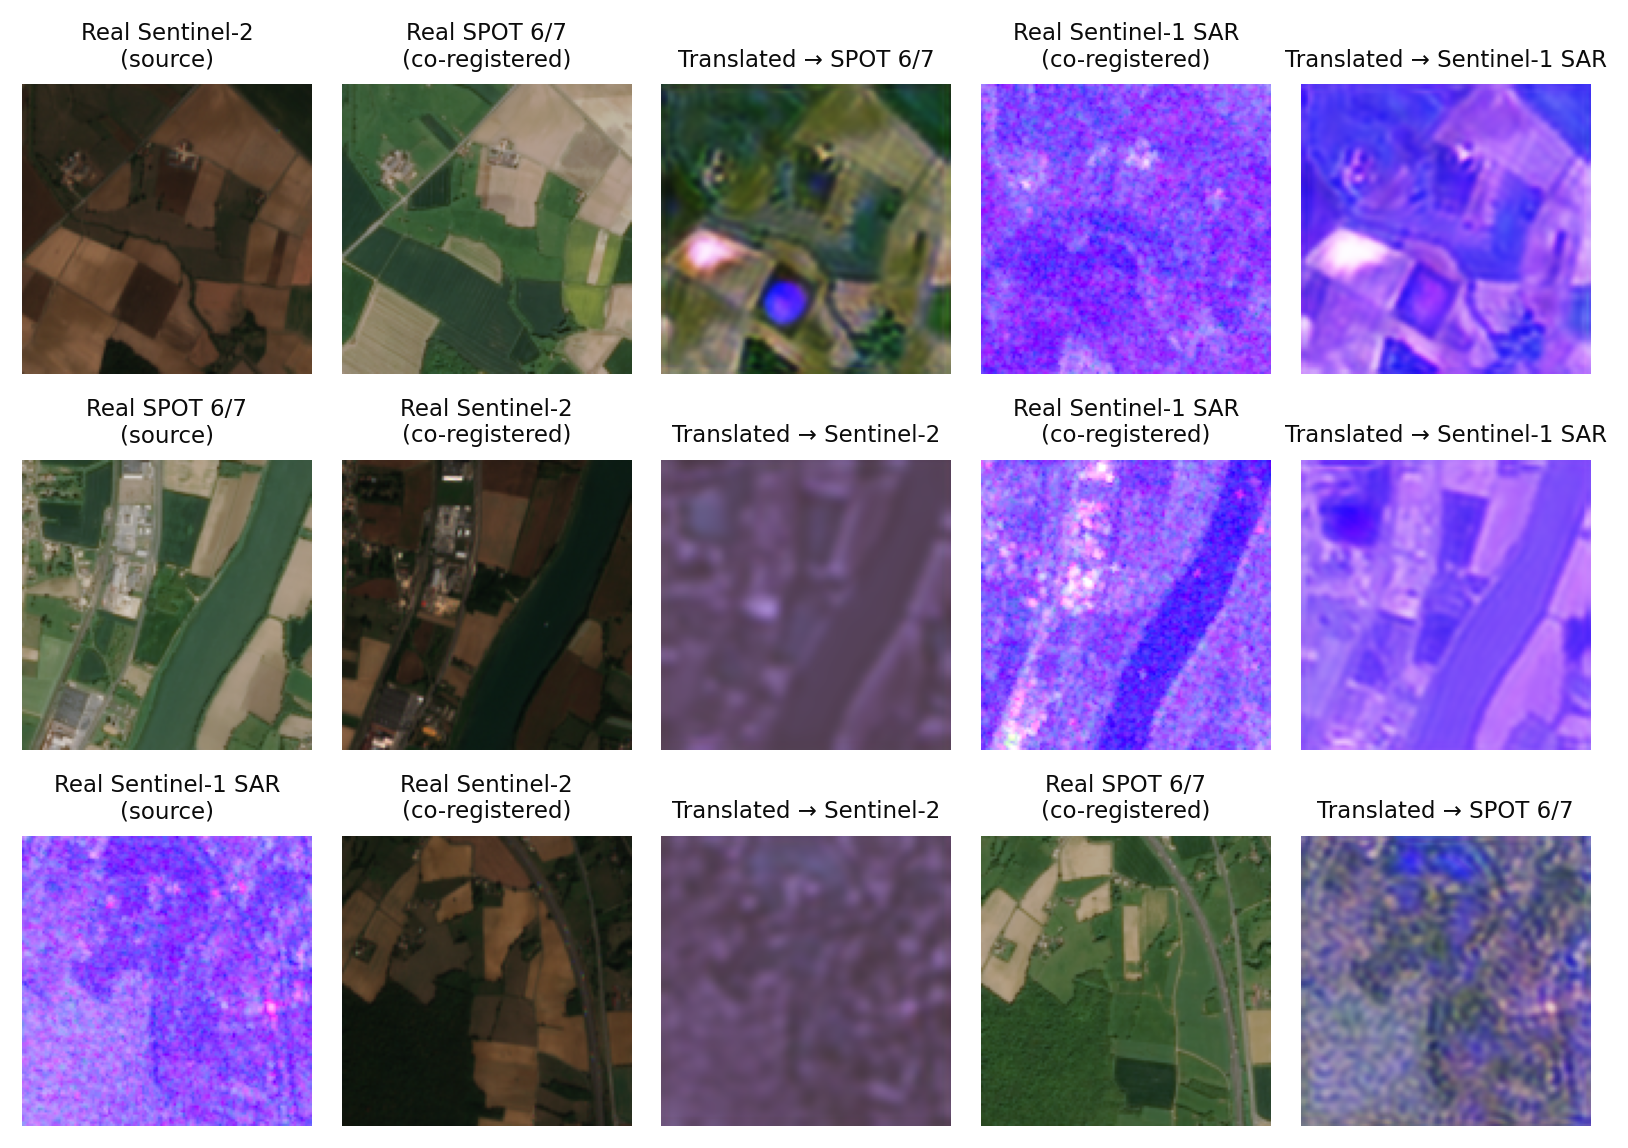
\includegraphics[width=0.7\textwidth]{figures/fig_paired_translation.png}
\caption{Translations of one held-out patch per source domain (first column of each row) into the two other domains, next to the real co-registered patch of each target domain. The style is the centroid embedding of the target domain, and the patches were chosen by a fixed random seed before inspection. Sentinel-1 patches are displayed as VV, VH, and the saturated difference channel in red, green, and blue.}
\label{fig:paired}
\end{figure*}

\begin{table}[t]
\centering
\caption{Translation into each target on held-out patches. PSNR (dB) against the co-registered real target patch for the translation, for the copied source (Copy) and for a constant target-mean image (Const.); Style is the share of outputs that the encoder assigns to the target domain; Edge is the edge-map correlation with the source.}
\label{tab:gen}
\footnotesize
\setlength{\tabcolsep}{3.5pt}
\begin{tabular}{@{}lccccc@{}}
\toprule
\textbf{Pair} & \textbf{Transl.} & \textbf{Copy} & \textbf{Const.} & \textbf{Style} & \textbf{Edge} \\
\midrule
S2 $\rightarrow$ SPOT   & 14.6 & 13.1 & 17.2 & 57\% & 0.82 \\
S2 $\rightarrow$ SAR    & 14.6 & 5.7 & 20.5 & 18\% & 0.87 \\
SPOT $\rightarrow$ S2   & 13.5 & 13.1 & 17.8 & 29\% & 0.71 \\
SPOT $\rightarrow$ SAR  & 16.8 & 7.4 & 20.5 & 80\% & 0.82 \\
SAR $\rightarrow$ S2    & 13.3 & 5.7 & 17.8 & 12\% & 0.94 \\
SAR $\rightarrow$ SPOT  & 13.0 & 7.4 & 17.2 & 45\% & 0.92 \\
\bottomrule
\end{tabular}
\end{table}

The style vector is used: the PSNR for the source to translation is higher than for the source to the real target domain (by 3.3 to 7.6~dB) for 5 of 6 pairs, and parcels are still recognizable in the figure, even though the road is not. The target radiometry is not reproduced: the constant image is correlated better with the real target patch than the translation for all 6 pairs (by 2.6 to 5.9~dB; the correlation is always higher than 0.61, better for pairs involving SAR than for others), the encoder assigns the outputs to the target domain in only 12\% to 80\% of the cases, and translations into Sentinel-2 are a blurred purple-gray haze whose channel means are equal within 0.001 for all 3 sources, and much brighter than real Sentinel-2 patches (by The identity mapping of Sentinel-2 is also not very well reproduced (13.7~dB, while for SPOT and SAR 20.3~dB and 24.3~dB, respectively); Sentinel-2 is the least strong of the generator both as source and as target. The different modalities acquired at different times constrained the degree to which the pixels may be matched, but did not account for the poorer transmission of a constant image.

The style space of the two points was sampled by interpolating between the two domain centroids, $z(\alpha)=(1-\alpha)\bar z_a+\alpha\bar z_b$ with the points renormalized to unit length, for 300 sets of source patches. The two pairs involving SAR resulted in a smooth change in output, close to linear (linearity ratio 0.91 and 0.96, monotone for 96\% and 100\% of the patches, respectively). The change is 10\% smaller for Sentinel-2 and SPOT, and only the first step ($0<\alpha<0.25$) contains the majority of the change 89\% of the patches, with only 41\% of them being monotone. There are 1.59~M parameters for the generator and 0.89~M for the encoder, and the CPU takes approximately 84~ms for a translation per patch.

Fig.~\ref{fig:interp} shows this interpolation for one held-out SPOT~6/7 source patch.

\begin{figure}[t]
\centering
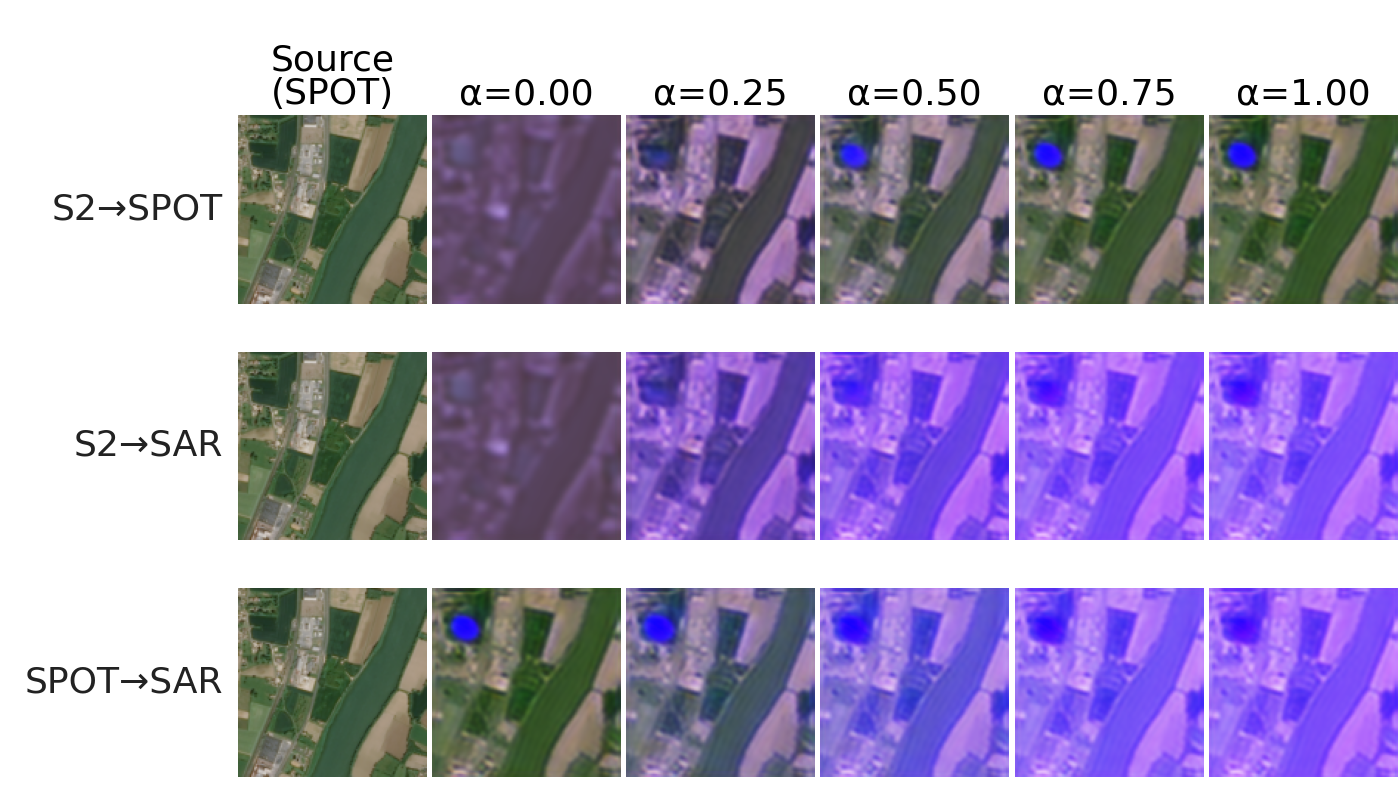
\includegraphics[width=\columnwidth]{figures/fig_interp_compact.png}
\caption{Interpolation of the style vector between two domain centroids, $z(\alpha)=(1-\alpha)\bar z_a+\alpha\bar z_b$ renormalized to unit length, applied to one held-out SPOT~6/7 source patch (first column). Each row is a pair of domains $a \rightarrow b$ and $\alpha$ runs from the style of $a$ ($\alpha=0$) to the style of $b$ ($\alpha=1$). The patch was chosen by a fixed random seed before inspection.}
\label{fig:interp}
\end{figure}

The architectural objectives of Table~\ref{tab:gap} are achieved: there is no labeling of the domain, a single generator for all the ordered pairs of three domains, and a continuous 64-dimensional domain code. None of the cited methods were trained on the same data as used for this work, and the numbers published for these methods are from other data and tasks, so any comparison to the quality of the result is not warranted, and no claim is made that the approach is better than SS(DA)$^2$, StarGAN~v2, or any of the other methods.

\section{Limitations}
\label{sec:limitations}
The above results have some restrictions. First, the held-out patches are from one Sentinel-2 tile, and the training set is largely from two other tiles, and so the results are a blend of model quality and a shift towards a different region; domain centroids are from different regions to the patches they're applied to. Second, there is no simultaneous modality, limiting the ability to agree at the pixel level with the co-registered reference, and there are artifacts in the preprocessing (saturated SAR channel and synthetic fourth SPOT channel). Third, for each model, the training was performed only once on a CPU with only 12 epochs of the generator and 10 epochs of the encoder (Sec.~\ref{sec:setup}), and the training loops were not seeded, no run-to-run variation was tested, no ablation of the six generator losses was performed, and no other method of translation was trained on the same data. Fourth, PSNR and SSIM are used for the degree of agreement with a co-registered image, not for realism, and the rate of style transfer is evaluated by the same encoder used for conditioning the generator. Fifth, only three sensor domains, one geographic setting and 1,500 of 2,433 locations were utilized; the larger MSC-France corpus that was foreseen forencoder pretraining and the angle-conditioning were not used. Finally, generalisation of unseen sensor pairs and downstream accuracy are not assessed.

\section{Conclusion and Future Work}
The proposed framework was a novel multi-domain self-supervised adaptation framework for satellite-based image data, which consisted of two main components: a contrastive domain encoder for learning label-free, continuous embeddings of the sensor style of the images, and an AdaIN-conditioned generator for generating an image in an arbitrary target style, given a source patch and its learned embedding from the domain encoder. The framework has the potential to comply with the design goals at the architectural level: No domain labels, one model for all ordered domain pairs, a continuous domain code, trained on real PASTIS-HD imagery (Sentinel-2, SPOT~6/7, Sentinel-1 SAR). There is a limited measured quality: the encoder identifies the sensor moderately (65.8\% vs 33.3\% chance) and the generator preserves the structure of the scene and uses the style vector, but cannot reproduce the radiometry of the measured sensor; translations into Sentinel-2 do not work.

Future work will involve (i) replacing the augmented-view positives with sensor-aware positive pairs based on spatial and temporal proximity and pretraining on a larger corpus MSC-France; (ii) fixing data issues found here, including all PASTIS-HD patches, a tile-stratified split and temporally matched acquisitions, a non-saturating SAR channel; (iii) training wider networks longer on a GPU with seeded runs, loss ablations and same-data baselines; and (iv) testing leave-one-domain-pair-out and zero-shot (SpaceNet~6) generalization and downstream crop classification and segmentation.

\bibliographystyle{IEEEtran}
\bibliography{references}

\end{document}
"
% Camera-ready build (authors shown): pdflatex main.tex
\ifdefined\ANON
\author{
\IEEEauthorblockN{Anonymous Authors}
\IEEEauthorblockA{Anonymous Affiliation}
}
\else
\author{
\IEEEauthorblockN{Shivangi\textsuperscript{1}, Benedict Tephila M.\textsuperscript{2}, Naveen J.\textsuperscript{3}}
\IEEEauthorblockA{
Department of Computer Science and Engineering \\
CHRIST (Deemed to be University), Bangalore -- 560029, India \\
\textsuperscript{1}shivangi.a@mtech.christuniversity.in,
\textsuperscript{2}benedict.tephila@christuniversity.in,
\textsuperscript{3}naveen.j@christuniversity.in}
}
\fi

\maketitle

\begin{abstract}
The performance of deep learning models trained for the analysis of satellite images suffers when the same land-cover classes are captured by a different sensor, at a different season, or in a different region. Current domain-adaptation techniques typically require labeled target data, a fixed domain library, or both, but these are hard to obtain with evolving and expanding multi-sensor archives. Firstly, we present a continuous domain encoder that produces a label-free style embedding from unlabeled multi-sensor patches through the use of a contrastive (InfoNCE) pretext task, and secondly, we introduce a unified conditional generator that creates a style conditioned transformation of the content of the source patch into an arbitrary style of the target domain by learning a style embedding as a continuous latent space rather than a discrete class label. Both networks trained on 1,200 patches per sensor provided by PASTIS-HD (Sentinel-2, SPOT~6/7, Sentinel-1 SAR) and tested on 300 held-out patches per sensor from a region that is mostly different. The encoder successfully completes its pretext task, but recognises the sensor with only some success (65.8\% as opposed to 33.3\% chance). The generator maintains the scene structure and performs well on the pairs that contain SAR, but does not reproduce the radiometry of the target sensor: a constant image is closer to the actual target patch than a translation, and translated images end up as a source-independent color cast, when SAR is present in one of the pairs. This paper does not include generalization to unseen sensor pairs, nor does it include downstream accuracy.
\end{abstract}

\begin{IEEEkeywords}
domain adaptation, self-supervised learning, generative adversarial networks, contrastive learning, multi-sensor satellite imagery, image-to-image translation
\end{IEEEkeywords}

\section{Introduction}

Satellite remote sensing has now evolved from one single mission to a constellation of optical and radar satellites, seeing the Earth's surface together and in succession, such as Sentinel-2, Landsat, SPOT and a growing number of commercial very-high-resolution (VHR) and synthetic aperture radar (SAR) satellites. The use of deep learning models for land-cover classification, crop mapping and change detection has been increasingly placed on the ability to perform on this multi-sensor heterogeneous archive, as opposed to the single sensor they were trained on.

It is hard to achieve this cross-sensor requirement in practice. These include different radiometric calibration, spectral response, spatial resolution, and noise properties for each sensor, which vary from atmospheric haze and calibration drift in optical imagery to speckle noise and incidence-angle-dependent backscatter in SAR. Consequently, a model trained with the statistics from one sensor may exhibit a dramatic decrease in accuracy when applied to another sensor, even when the land-cover classes are the same. Modeling often requires the adaptation to a new domain with little or no target domain labeled data because of the high cost of acquiring and annotating imagery from all sensors of interest.

The current methods can be classified into two families. Satellite-specific methods, like multi-source standardization~\cite{tasar2020standardgan} normalize translation on a discrete domain identity that is manually assigned to each satellite and are claimed to have difficulty with unseen combinations of domains. However, self-supervised methods like SS(DA)$^2$~\cite{zhang2023ssdada} do not require labels or an explicit domain boundary and only translate between two satellites at a time, meaning that a new method must be developed for each new pair of satellites. In the general image-translation literature, StarGAN~\cite{choi2018stargan} and StarGAN~v2~\cite{choi2020starganv2} integrate a multitude of domains into a single generator, with StarGAN~v2 additionally using a continuous style code, and performing regular evaluations on natural images. Diffusion-based translators~\cite{vinholi2024multisensor,kieu2025universal} are more faithful but work on discrete domain sets, with higher inference cost.

The combination of label-free training, a continuous (discretely labeled is not the only option) representation of the domain and a single generator that can translate into an arbitrary target style is not yet explicitly provided in the literature for satellite images. It is the motivation for the present work to fill this gap.

The first two properties are addressed by further developing the pairwise approach of the SS(DA)$^2$ paradigm to a continuous, StarGAN~v2-style unified generator without the need for any domain-specific conditioning: A domain encoder produces a uniform embedding of the domain characteristics of each patch, and a single generator, modulated by the embedding through the use of AdaIN, maps a source patch to the domain of any target patch's embedding. These two components are designed, implemented, and evaluated using held-out data, which is not covered by this paper.

This paper makes the following contributions:
\begin{itemize}
\item A self-supervised contrastive domain encoder to generate label-free, continuous embeddings of sensor/style features from unlabeled multi-sensor patches.
A single AdaIN-modulated conditional generator conditioned on this embedding, instead of a discrete domain code, so no retraining per domain pair is required for the translation to an arbitrary target style.
An objective for six terms of training that maintains the geospatial content while changing the style of the content.
\item held out evaluation on real PASTIS-HD data that reports what works (label-free continuous embeddings, structure preserving, style conditioned translation) and what doesn't (moderate sensor information in the embedding, target radiometry not reproduced).
\end{itemize}

\section{Related Work}

\subsection{Domain Adaptation for Satellite Imagery}
StandardGAN~\cite{tasar2020standardgan} is used to standardize each source domain towards a common reference for semantic segmentation of multi-source VHR satellite images towards the common reference. It works on a set of discrete and enumerated domains, and according to the report of its authors, it has trouble maintaining the content of the images and it has poor generalisation ability with respect to sensor combinations not encountered at the time of standardisation. SS(DA)$^2$~\cite{zhang2023ssdada} does not require labeled target data or the domain boundary: a contrastive, domain-agnostic GAN translates between two satellite domains with unlabeled images. The downside to this, and what is being solved here, is that it is pairwise: each model can accommodate only two satellites.

\subsection{Multi-Domain Image-to-Image Translation}
StarGAN~\cite{choi2018stargan} combined multi-domain translation into a single generator, and used a discrete one-hot domain vector as the condition. It is replaced in StarGAN~v2~\cite{choi2020starganv2} by a continuous style code from a mapping network or style encoder fed into AdaIN~\cite{huang2017adain} and it is evaluated on natural image datasets, using realism metrics (e.g., FID), and not on satellite imagery. Multi-sensor optical image translation~\cite{vinholi2024multisensor} and universal multi-domain routing~\cite{kieu2025universal} are both based on diffusion and enhance fidelity, but the router still chooses from a discrete set of domain experts and iterative sampling is more expensive than one feed-forward GAN pass, especially for large mosaics of satellites.

\section{Research Gap and Motivation}
The most similar methods are compared to the properties targeted here in Table~\ref{tab:gap}. SS(DA)$^2$ is label-free and pairwise while StarGAN~v2 is continuous domain representation and supervised discrete domain identity at training time, and designed for remote sensing; StandardGAN is designed for satellite imagery and requires discrete domain identity. All the methods reviewed here did not accept labels and used a continuous domain without a generator specifically designed for and tested on satellite images. This project's goals, ~1 and ~2, are specifically aimed at this combination: Continuous domain encoder without labels, and a single generator conditioned on its embedding.

\begin{table}[t]
\centering
\caption{Qualitative comparison of properties relevant to the identified research gap.}
\label{tab:gap}
\resizebox{\linewidth}{!}{%
\begin{tabular}{@{}lccc@{}}
\toprule
\textbf{Method} & \textbf{Label-free} & \textbf{Continuous domain repr.} & \textbf{Satellite-specific} \\
\midrule
StandardGAN~\cite{tasar2020standardgan}    & \ding{55} & \ding{55} & \ding{51} \\
SS(DA)$^2$~\cite{zhang2023ssdada}          & \ding{51} & \ding{55} (pairwise) & \ding{51} \\
StarGAN~\cite{choi2018stargan}             & \ding{55} & \ding{55} & \ding{55} \\
StarGAN~v2~\cite{choi2020starganv2}        & \ding{55} & \ding{51} & \ding{55} \\
\textbf{Proposed (Objectives 1--2)}        & \ding{51} & \ding{51} & \ding{51} \\
\bottomrule
\end{tabular}}
\end{table}

\section{Proposed Methodology}

\begin{figure*}[t]
\centering
\resizebox{\textwidth}{!}{%
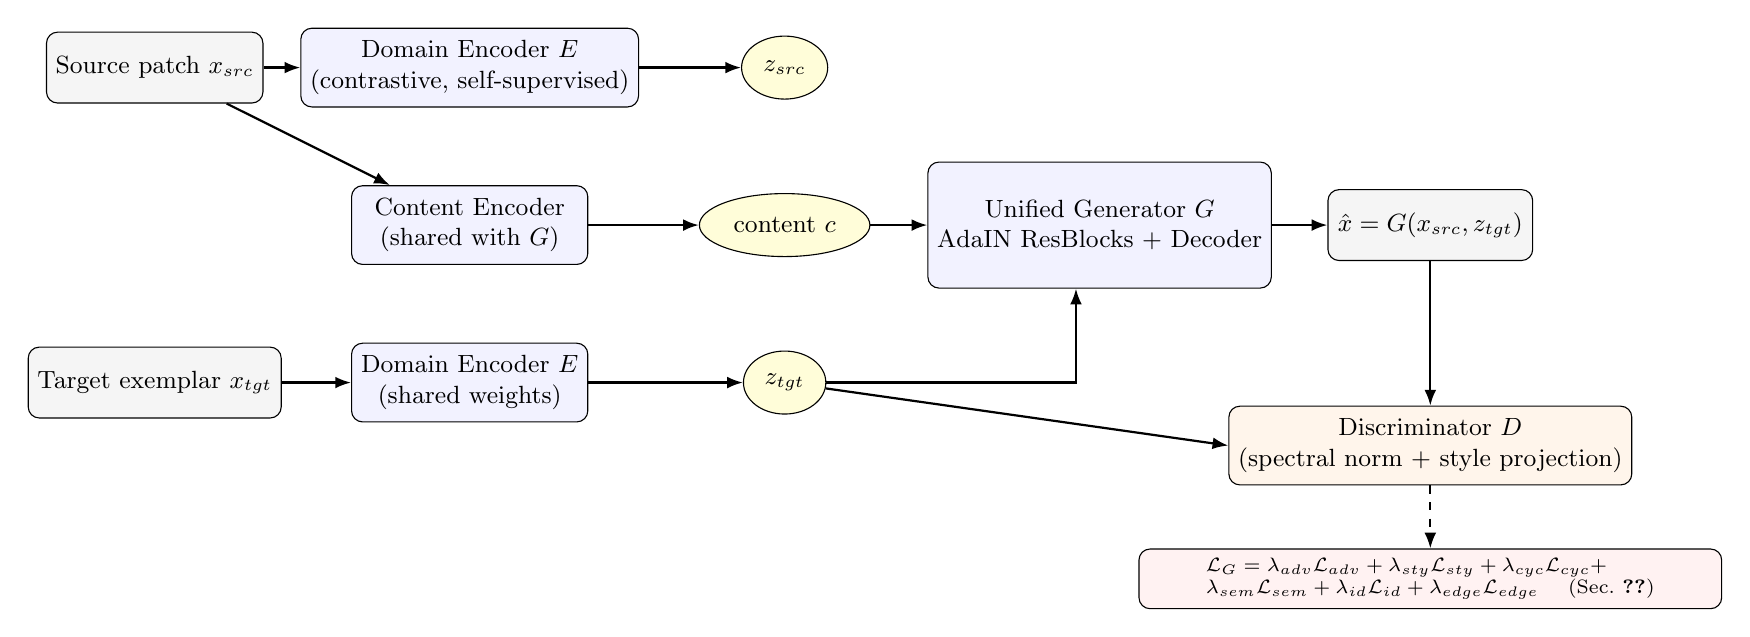
\begin{tikzpicture}[
  node distance=8mm and 10mm,
  box/.style={draw, rounded corners, align=center, minimum height=1.0cm, font=\small, fill=blue!5},
  data/.style={draw, rounded corners, align=center, minimum height=0.9cm, font=\small, fill=gray!8},
  vec/.style={draw, ellipse, align=center, minimum height=0.8cm, font=\small, fill=yellow!15},
  lossbox/.style={draw, rounded corners, align=left, font=\scriptsize, fill=red!5},
  arr/.style={-{Latex[length=2mm]}, thick}
]
  \node[data]                              (xsrc) at (0,6)    {Source patch $x_{src}$};
  \node[data]                              (xtgt) at (0,2)    {Target exemplar $x_{tgt}$};

  \node[box, minimum width=3.0cm]          (E1)   at (4.0,6)  {Domain Encoder $E$\\(contrastive, self-supervised)};
  \node[box, minimum width=3.0cm]          (CE)   at (4.0,4)  {Content Encoder\\(shared with $G$)};
  \node[box, minimum width=3.0cm]          (E2)   at (4.0,2)  {Domain Encoder $E$\\(shared weights)};

  \node[vec]                               (zsrc) at (8.0,6)  {$z_{src}$};
  \node[vec]                               (c)    at (8.0,4)  {content $c$};
  \node[vec]                               (ztgt) at (8.0,2)  {$z_{tgt}$};

  \node[box, minimum width=3.2cm, minimum height=1.6cm] (G) at (12.0,4) {Unified Generator $G$\\AdaIN ResBlocks + Decoder};

  \node[data, minimum width=2.6cm]         (xfake) at (16.2,4) {$\hat{x} = G(x_{src}, z_{tgt})$};

  \node[box, fill=orange!8, minimum width=3.0cm] (D) at (16.2,1.2) {Discriminator $D$\\(spectral norm + style projection)};

  \draw[arr] (xsrc) -- (E1);
  \draw[arr] (xsrc) -- (CE);
  \draw[arr] (xtgt) -- (E2);
  \draw[arr] (E1) -- (zsrc);
  \draw[arr] (CE) -- (c);
  \draw[arr] (E2) -- (ztgt);
  \draw[arr] (c) -- (G);
  \draw[arr] (ztgt.east) -| ([xshift=-3mm]G.south);
  \draw[arr] (G) -- (xfake);
  \draw[arr] (xfake) -- (D);
  \draw[arr] (ztgt) -- (D.west);

  \node[lossbox, below=8mm of D, minimum width=7.4cm] (losses) {
    $\mathcal{L}_G = \lambda_{adv}\mathcal{L}_{adv} + \lambda_{sty}\mathcal{L}_{sty} + \lambda_{cyc}\mathcal{L}_{cyc} +$\\
    $\lambda_{sem}\mathcal{L}_{sem} + \lambda_{id}\mathcal{L}_{id} + \lambda_{edge}\mathcal{L}_{edge}$ \quad (Sec.~\ref{sec:objective})
  };
  \draw[arr, dashed] (D.south) -- (losses.north);
\end{tikzpicture}}
\caption{Simplified architecture of the two components reported here: the self-supervised domain encoder $E$ (Sec.~\ref{sec:encoder}) and the AdaIN-conditioned generator $G$ with projection discriminator $D$ (Sec.~\ref{sec:generator}). The source embedding $z_{src}$ is reused in two further passes through $G$, omitted for clarity, for the cycle and identity losses of Sec.~\ref{sec:objective}.}
\label{fig:architecture}
\end{figure*}

The two components that are addressed in this paper are shown in Fig.~\ref{fig:architecture}. A domain encoder $E$ is used to project an unlabeled image patch to a continuous style embedding, a content encoder $G$ is used as the downsampling path of the generator to extract a domain-invariant spatial content code, and a unified generator $G$ is used to combine the content of a source patch with the embedding of a target patch to generate a translation, which is then evaluated by a projection discriminator $D$.

\subsection{Self-Supervised Continuous Domain Encoder}
\label{sec:encoder}
This is achieved by the encoder $E_\theta$ which maps an $H \times W$ patch containing $C$ channels (4 in this implementation, corresponding to 3 optical channels and 1 auxiliary channel, see Sec.~\ref{sec:dataset}) to a continuous embedding $z \in \mathbb{R}^{64}$. The network is composed of an input-adapter convolution, followed by three stride-2 convolutional blocks (Conv--InstanceNorm--LeakyReLU) to gradually reduce the spatial resolution, but expand the channel width, followed by a squeeze-and-excitation (SE) block~\cite{hu2018senet} which recalibrates the responses channel-wise.

Instead of pooling to a class score, the encoder calculates two types of statistics, the first-order mean $\mu$ and the second-order standard deviation $\sigma$ of the final feature map, representing the radiometric and textural style of the patch, respectively, without relying on spatial content:
\begin{equation}
\mu_c = \frac{1}{HW}\sum_{i,j} h_{c,i,j}, \qquad
\sigma_c = \sqrt{\frac{1}{HW}\sum_{i,j}(h_{c,i,j}-\mu_c)^2 + \epsilon}
\label{eq:stats}
\end{equation}
where $h$ is the feature map after the SE block. The concatenated statistics $[\mu;\sigma]$ (optionally fused with a projected acquisition-angle feature when angle metadata is available, unused in the sensor-only experiment reported here) are passed through a multilayer perceptron projection head and L2-normalized onto the unit hypersphere:
\begin{equation}
z = \frac{f_\phi([\mu;\sigma])}{\lVert f_\phi([\mu;\sigma]) \rVert_2}, \qquad z \in \mathbb{R}^{64}.
\label{eq:embed}
\end{equation}

The encoder is pretrained with no domain labels using a contrastive pretext task in the style of InfoNCE~\cite{oord2018cpc}. Two independently augmented views ($z_1, z_2$) of the same patch (random flips and 90\textdegree{} rotations) are treated as a positive pair, and all other patches in the training batch act as negatives:
\begin{equation}
\mathcal{L}_{con} = -\frac{1}{2B}\sum_{i=1}^{B}\Big[
\log\frac{e^{\,z_{1,i}\cdot z_{2,i}/\tau}}{\sum_{j} e^{\,z_{1,i}\cdot z_{2,j}/\tau}}
+
\log\frac{e^{\,z_{2,i}\cdot z_{1,i}/\tau}}{\sum_{j} e^{\,z_{2,i}\cdot z_{1,j}/\tau}}
\Big]
\label{eq:infonce}
\end{equation}
where $B$ is the batch size and $\tau$ is a temperature hyperparameter. Because positives and negatives come from augmentation rather than sensor labels, no supervision of domain identity is used, and any patch can be projected into the same continuous space at inference time.

\subsection{Unified Conditional Generator}
\label{sec:generator}
The generator $G_\psi$ takes a source patch $x_{src}$ and a target embedding $z_{tgt}$ (produced by the frozen encoder $E$ on a target-domain exemplar) and synthesizes a translated patch $\hat{x} = G_\psi(x_{src}, z_{tgt})$. A single generator instance is shared across all domains: the target style is entirely determined by $z_{tgt}$, so translation into any domain the encoder can embed -- rather than only domains enumerated at training time -- requires no architectural change or additional parameters.

The content path follows an encoder-bottleneck-decoder design in the spirit of StarGAN~v2~\cite{choi2020starganv2}, adapted to be label-free. A content encoder with reflection-padded convolutions and instance normalization downsamples $x_{src}$ to a domain-invariant content code $c = \mathrm{Enc}_c(x_{src})$. This code is passed through four residual blocks modulated by Adaptive Instance Normalization (AdaIN)~\cite{huang2017adain}, which injects the target style at every block:
\begin{equation}
\mathrm{AdaIN}(h, z) = \gamma(z)\cdot\frac{h - \mu(h)}{\sigma(h)} + \beta(z)
\label{eq:adain}
\end{equation}
where $\mu(h), \sigma(h)$ are the per-channel instance statistics of the intermediate feature map $h$, and $\gamma(z) = W_\gamma z + b_\gamma$, $\beta(z) = W_\beta z + b_\beta$ are affine parameters regressed from the continuous embedding. The decoder mirrors the encoder with two AdaIN-modulated upsampling stages; bilinear (rather than nearest-neighbor or transposed-convolution) upsampling is used to avoid checkerboard artifacts, followed by a reflection-padded output convolution with a $\tanh$ activation.

\subsection{Discriminator with Continuous Style Projection}
The discriminator $D_\xi$ is a multi-scale PatchGAN with spectral normalization~\cite{miyato2018spectral} applied to every convolutional layer, which stabilizes adversarial training by bounding the Lipschitz constant of each layer. In addition to an unconditional real/fake head, $D_\xi$ projects its intermediate features onto the conditioning embedding $z$:
\begin{equation}
D_\xi(x, z) = D_{uncond}(x) + \frac{\langle \phi(x), W_{proj}\,z\rangle}{\sqrt{d}}
\label{eq:disc}
\end{equation}
where $\phi(x)$ is the discriminator's penultimate feature map, $W_{proj}$ is a learned linear projection of the embedding, and $d$ is the feature dimension. This term penalizes translations whose visual style does not match the conditioning embedding $z$, complementing the encoder's own style-reconstruction signal (Sec.~\ref{sec:objective}).

\subsection{Composite Training Objective}
\label{sec:objective}
The generator is trained with a weighted sum of six loss terms, each targeting a specific failure mode observed in unconstrained multi-domain translation:

\emph{Adversarial loss} (least-squares GAN~\cite{mao2017lsgan}), encouraging $\hat{x}$ to be indistinguishable from real target-domain patches under the style-conditioned discriminator:
\begin{align}
\mathcal{L}_D &= \tfrac{1}{2}\mathbb{E}\big[(D_\xi(x_{tgt}, z_{tgt}) - 1)^2\big] + \tfrac{1}{2}\mathbb{E}\big[D_\xi(\hat{x}, z_{tgt})^2\big] \\
\mathcal{L}_{adv} &= \mathbb{E}\big[(D_\xi(\hat{x}, z_{tgt}) - 1)^2\big]
\label{eq:adv}
\end{align}

\emph{Style-reconstruction loss}, requiring the target style to be measurable in the output by re-encoding it:
\begin{equation}
\mathcal{L}_{sty} = \mathbb{E}\,\lVert E(\hat{x}) - z_{tgt} \rVert_1
\label{eq:sty}
\end{equation}

\emph{Cycle-consistency loss}~\cite{zhu2017cyclegan}, translating $\hat{x}$ back toward the source style and requiring recovery of the original patch, which discourages mode collapse across domains:
\begin{equation}
\mathcal{L}_{cyc} = \mathbb{E}\,\lVert G(\hat{x}, z_{src}) - x_{src} \rVert_1
\label{eq:cyc}
\end{equation}

\emph{Semantic-preservation loss}, penalizing drift in the domain-invariant content code between the source and the translation, so that geospatial layout (parcel boundaries, roads) is not altered by the style change:
\begin{equation}
\mathcal{L}_{sem} = \mathbb{E}\,\lVert \mathrm{Enc}_c(\hat{x}) - \mathrm{Enc}_c(x_{src}) \rVert_1
\label{eq:sem}
\end{equation}

\emph{Identity loss}, requiring that conditioning the generator on the source's own style leaves the patch unchanged:
\begin{equation}
\mathcal{L}_{id} = \mathbb{E}\,\lVert G(x_{src}, z_{src}) - x_{src} \rVert_1
\label{eq:id}
\end{equation}

\emph{Edge-preservation loss}, comparing Sobel gradient magnitudes between $\hat{x}$ and $x_{src}$ to keep agricultural parcel boundaries and road edges sharp:
\begin{equation}
\mathcal{L}_{edge} = \mathbb{E}\,\lVert \nabla_{Sobel}(\hat{x}) - \nabla_{Sobel}(x_{src}) \rVert_1
\label{eq:edge}
\end{equation}

The total generator objective is
\begin{align}
\mathcal{L}_G ={}& \lambda_{adv}\mathcal{L}_{adv} + \lambda_{sty}\mathcal{L}_{sty} + \lambda_{cyc}\mathcal{L}_{cyc} \notag \\
& + \lambda_{sem}\mathcal{L}_{sem} + \lambda_{id}\mathcal{L}_{id} + \lambda_{edge}\mathcal{L}_{edge}
\label{eq:total}
\end{align}
with weights listed in Table~\ref{tab:hyperparams}. The framework additionally defines a geometric (SSIM-style) preservation loss $\mathcal{L}_{geo}$, activated when either the source or target domain is an off-nadir viewing-angle domain; because the PASTIS-HD experiment reported in Sec.~\ref{sec:results} uses only sensor domains, $\mathcal{L}_{geo}$ is inactive ($\lambda_{geo}\mathcal{L}_{geo}=0$) for the results shown here.

\section{Dataset and Preprocessing}
\label{sec:dataset}
Experiments are conducted on patches that are taken from PASTIS-HD~\cite{garnot2021panoptic,astruc2024omnisat} a public benchmark of $2{,}433$ co-registered agricultural-parcel locations in France for which SAR time series from Sentinel-2 and Sentinel-1 datasets are provided, and in the HD extension a very-high-resolution image from SPOT~6/7. A conversion pipeline matches up patches by identifier and exports a $128\times128$ 4-channel tensor per modality, per location: Sentinel-2 Red, Green, Blue and near-infrared channels are kept as is; SPOT~6/7 is resized from $1280\times1280$ and provided with a synthetic near-infrared proxy channel, and the two polarizations of Sentinel-1 (VV and VH) are extended with a derived ratio and average channel, and are converted from decibel to linear units. All modalities have the range of [-1,1]. In this experiment, the first $1{,}500$ locations per domain in identifier order (the patch cap of the pipeline) is converted from three Sentinel-2 tiles. In this case, 80\% of the patches are used as training data and 20\% are held out, with 1200 used in the training set and 300 held out, meaning that all held out patches are in a single region, only slightly underrepresented in training, and the evaluation is largely on a different region. The modalities are co-registered, but not simultaneous: the first Sentinel-1 acquisition is 11 days after the first Sentinel-2 acquisition (median) and the SPOT imagery is provided from 2019. After conversion, the SAR difference channel is saturated at $+1$ for 97.9\% of its values. Random flips, rotations by 90\textdegree{} and small Gaussian radiometric noise $\sigma \sim \mathcal{U}[0, 0.01]$ are added to the training patches.

\section{Experimental Setup}
\label{sec:setup}
It is implemented in Python~3.13 with PyTorch~$\geq$2.4 and is controlled by a single command line entry point, which first trains the domain-encoder, then trains the generator and discriminator jointly. All training and evaluation were performed on the CPU of a laptop with following specification: Intel Core i7-9750H, 6 core, 7.8~GB RAM. The width of the generator and discriminator (base width 32) is kept narrow to ensure this compute is tractable for training, rather than be close to a reported baseline. For the results in Sec.~\ref{sec:results} the following hyperparameters were used, as shown in Tab.~\ref{tab:hyperparams}.

\begin{table}[t]
\centering
\caption{Training hyperparameters.}
\label{tab:hyperparams}
\begin{tabular}{@{}ll@{}}
\toprule
\textbf{Stage 1 -- Domain Encoder} & \textbf{Value} \\
\midrule
Embedding dimension $d$            & 64 \\
Optimizer                          & AdamW \\
Learning rate                      & $5\times10^{-4}$ \\
Weight decay                       & $1\times10^{-4}$ \\
Contrastive temperature $\tau$     & 0.07 \\
Epochs                             & 10 \\
\midrule
\textbf{Stage 2 -- Generator / Discriminator} & \textbf{Value} \\
\midrule
Base channel width                 & 32 \\
Residual blocks                    & 4 \\
Optimizer ($G$, $D$)               & Adam ($\beta_1{=}0.5$, $\beta_2{=}0.999$) \\
Learning rate ($G$, $D$)           & $3\times10^{-4}$ \\
LR schedule                        & Cosine annealing, $\eta_{min}{=}10^{-5}$ \\
Gradient clipping (max norm)       & 1.0 \\
Epochs                             & 12 \\
Batch size                         & 8 \\
$\lambda_{adv},\lambda_{sty},\lambda_{id}$ & 1.0 each \\
$\lambda_{sem}$, $\lambda_{edge}$  & 2.0 each \\
$\lambda_{cyc}$                    & 10.0 \\
\bottomrule
\end{tabular}
\end{table}

\section{Results and Discussion}
\label{sec:results}
All results are on the 300 withheld patches per domain with a constant protocol and are only a single measurement from one trained model. Target domains are L2-normalized mean of the embedding of 1200 patches in the target domain, which are the \emph{centroid} of the domain (the training patches are used in the embedding process, but not for the evaluation step). The images are rescaled to $[0,1]$ against the co-registered real target patch, having two reference baselines: ``Copy'' for the untranslated source patch, and ``Const.'' for the constant image that corresponds to the mean of the target domain.

\subsection{Domain encoder (Objective~1)}
Table~\ref{tab:enc} summarizes the encoder. It achieves a solution to its contrastive task on held-out patches (loss 0.24 compared to 2.08 with an uninformative embedding; 88.2\% top-1 retrieval of the second view on 900 patches), while its embeddings are uniformly distributed over the hypersphere rather than in three concentrated clusters. They describe the sensor moderately: 65.8\% of held out patches are correctly assigned to the sensor by the nearest centroid as compared with 33.3\% randomly; the sensors overlap (silhouette coefficient 0.11); effective dimensionality is about 4. The co-registered patch of another sensor is retrieved at chance level, which means that the embedding does not contain information about the scene that is shared across sensors. One possible reason (not tested) is that instance discrimination does not include a term to group the patches of one sensor, and that proximity-based positive pairs as planned in the project plan were not used.

\begin{table}[t]
\centering
\caption{Domain encoder on 300 held-out patches per domain (S2: Sentinel-2).}
\label{tab:enc}
\begin{tabular}{@{}lc@{}}
\toprule
\textbf{Measurement} & \textbf{Result} \\
\midrule
Held-out InfoNCE loss (batch 8; chance 2.08)        & 0.24 \\
Top-1 instance retrieval among 900 patches          & 88.2\% \\
Nearest-centroid domain accuracy (chance 33.3\%)    & 65.8\% \\
\quad recall S2 / SPOT / SAR                        & 62.7 / 74.3 / 60.3\% \\
5-nearest-neighbor domain accuracy                  & 63.7\% \\
Cosine similarity within / between domains          & 0.32 / 0.04 \\
Silhouette coefficient (cosine distance)            & 0.11 \\
Participation ratio (of 64 dimensions)              & 3.85 \\
Same-location retrieval across sensors, top-1       & 0.3\% (chance 0.3\%) \\
\bottomrule
\end{tabular}
\end{table}

\subsection{Conditional generator (Objective~2)}
\begin{figure*}[t]
\centering
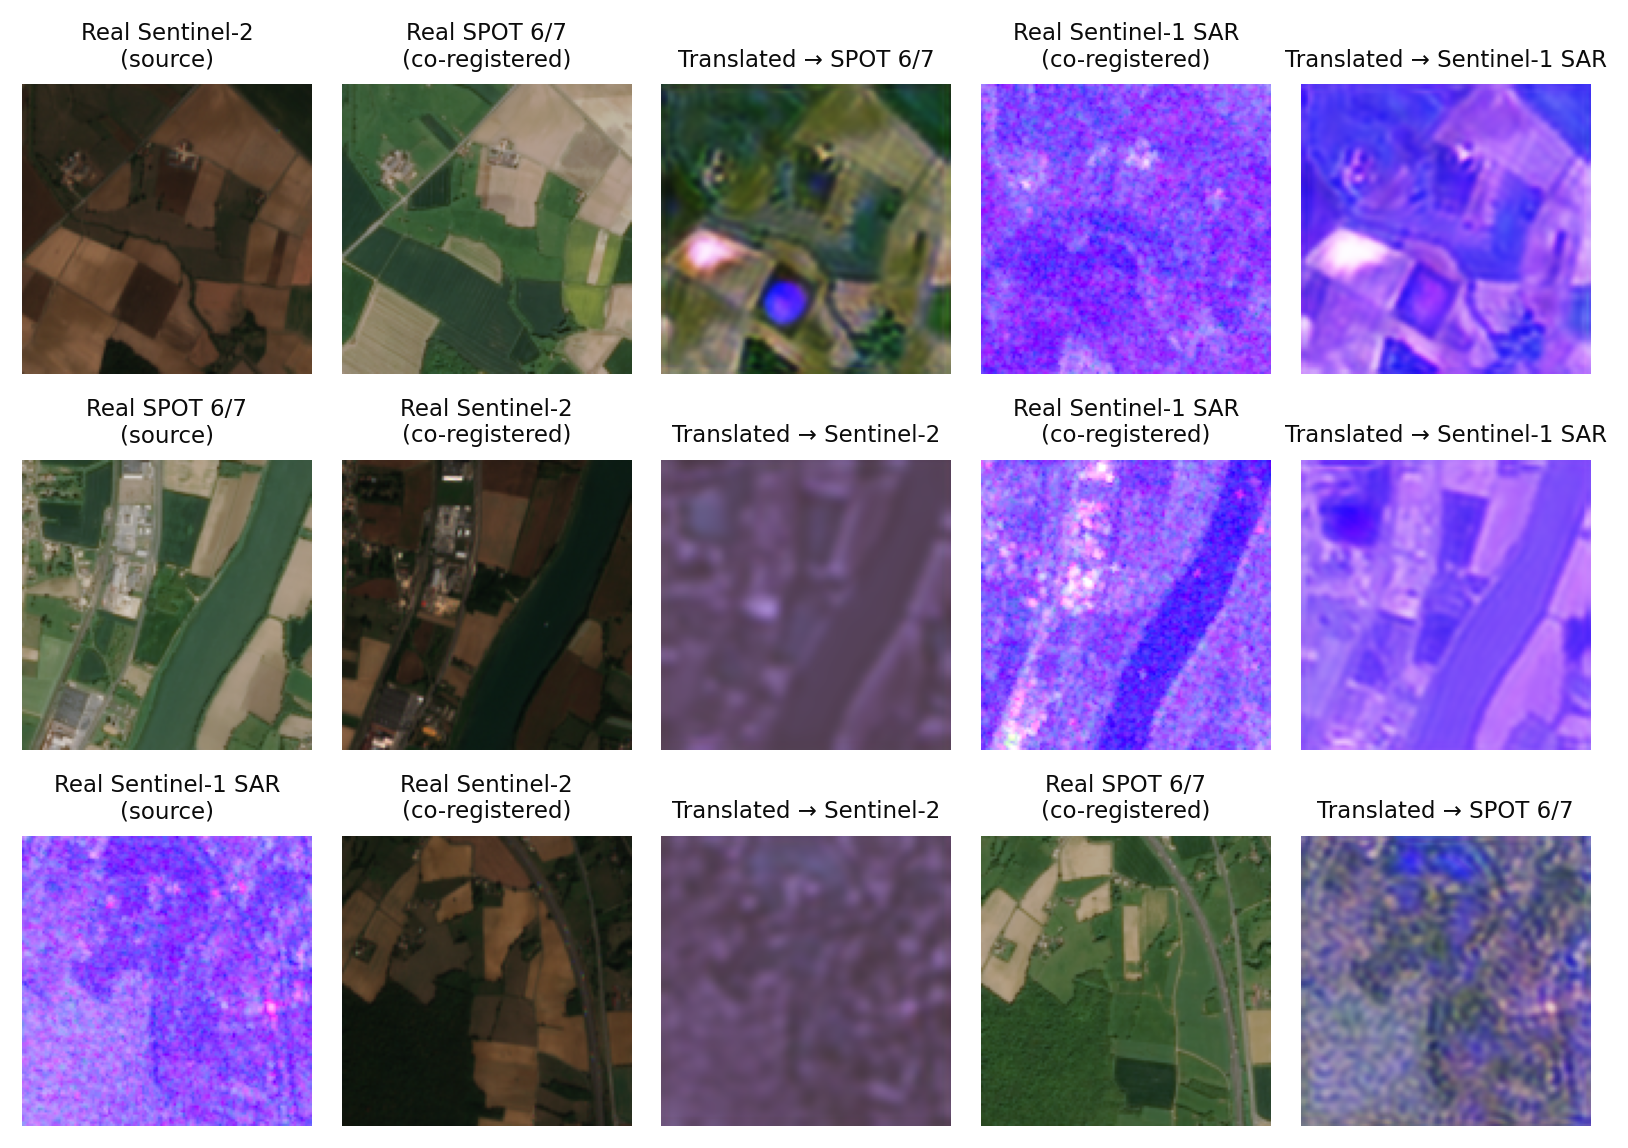
\includegraphics[width=0.7\textwidth]{figures/fig_paired_translation.png}
\caption{Translations of one held-out patch per source domain (first column of each row) into the two other domains, next to the real co-registered patch of each target domain. The style is the centroid embedding of the target domain, and the patches were chosen by a fixed random seed before inspection. Sentinel-1 patches are displayed as VV, VH, and the saturated difference channel in red, green, and blue.}
\label{fig:paired}
\end{figure*}

\begin{table}[t]
\centering
\caption{Translation into each target on held-out patches. PSNR (dB) against the co-registered real target patch for the translation, for the copied source (Copy) and for a constant target-mean image (Const.); Style is the share of outputs that the encoder assigns to the target domain; Edge is the edge-map correlation with the source.}
\label{tab:gen}
\footnotesize
\setlength{\tabcolsep}{3.5pt}
\begin{tabular}{@{}lccccc@{}}
\toprule
\textbf{Pair} & \textbf{Transl.} & \textbf{Copy} & \textbf{Const.} & \textbf{Style} & \textbf{Edge} \\
\midrule
S2 $\rightarrow$ SPOT   & 14.6 & 13.1 & 17.2 & 57\% & 0.82 \\
S2 $\rightarrow$ SAR    & 14.6 & 5.7 & 20.5 & 18\% & 0.87 \\
SPOT $\rightarrow$ S2   & 13.5 & 13.1 & 17.8 & 29\% & 0.71 \\
SPOT $\rightarrow$ SAR  & 16.8 & 7.4 & 20.5 & 80\% & 0.82 \\
SAR $\rightarrow$ S2    & 13.3 & 5.7 & 17.8 & 12\% & 0.94 \\
SAR $\rightarrow$ SPOT  & 13.0 & 7.4 & 17.2 & 45\% & 0.92 \\
\bottomrule
\end{tabular}
\end{table}

The style vector is used: the PSNR for the source to translation is higher than for the source to the real target domain (by 3.3 to 7.6~dB) for 5 of 6 pairs, and parcels are still recognizable in the figure, even though the road is not. The target radiometry is not reproduced: the constant image is correlated better with the real target patch than the translation for all 6 pairs (by 2.6 to 5.9~dB; the correlation is always higher than 0.61, better for pairs involving SAR than for others), the encoder assigns the outputs to the target domain in only 12\% to 80\% of the cases, and translations into Sentinel-2 are a blurred purple-gray haze whose channel means are equal within 0.001 for all 3 sources, and much brighter than real Sentinel-2 patches (by The identity mapping of Sentinel-2 is also not very well reproduced (13.7~dB, while for SPOT and SAR 20.3~dB and 24.3~dB, respectively); Sentinel-2 is the least strong of the generator both as source and as target. The different modalities acquired at different times constrained the degree to which the pixels may be matched, but did not account for the poorer transmission of a constant image.

The style space of the two points was sampled by interpolating between the two domain centroids, $z(\alpha)=(1-\alpha)\bar z_a+\alpha\bar z_b$ with the points renormalized to unit length, for 300 sets of source patches. The two pairs involving SAR resulted in a smooth change in output, close to linear (linearity ratio 0.91 and 0.96, monotone for 96\% and 100\% of the patches, respectively). The change is 10\% smaller for Sentinel-2 and SPOT, and only the first step ($0<\alpha<0.25$) contains the majority of the change 89\% of the patches, with only 41\% of them being monotone. There are 1.59~M parameters for the generator and 0.89~M for the encoder, and the CPU takes approximately 84~ms for a translation per patch.

Fig.~\ref{fig:interp} shows this interpolation for one held-out SPOT~6/7 source patch.

\begin{figure}[t]
\centering
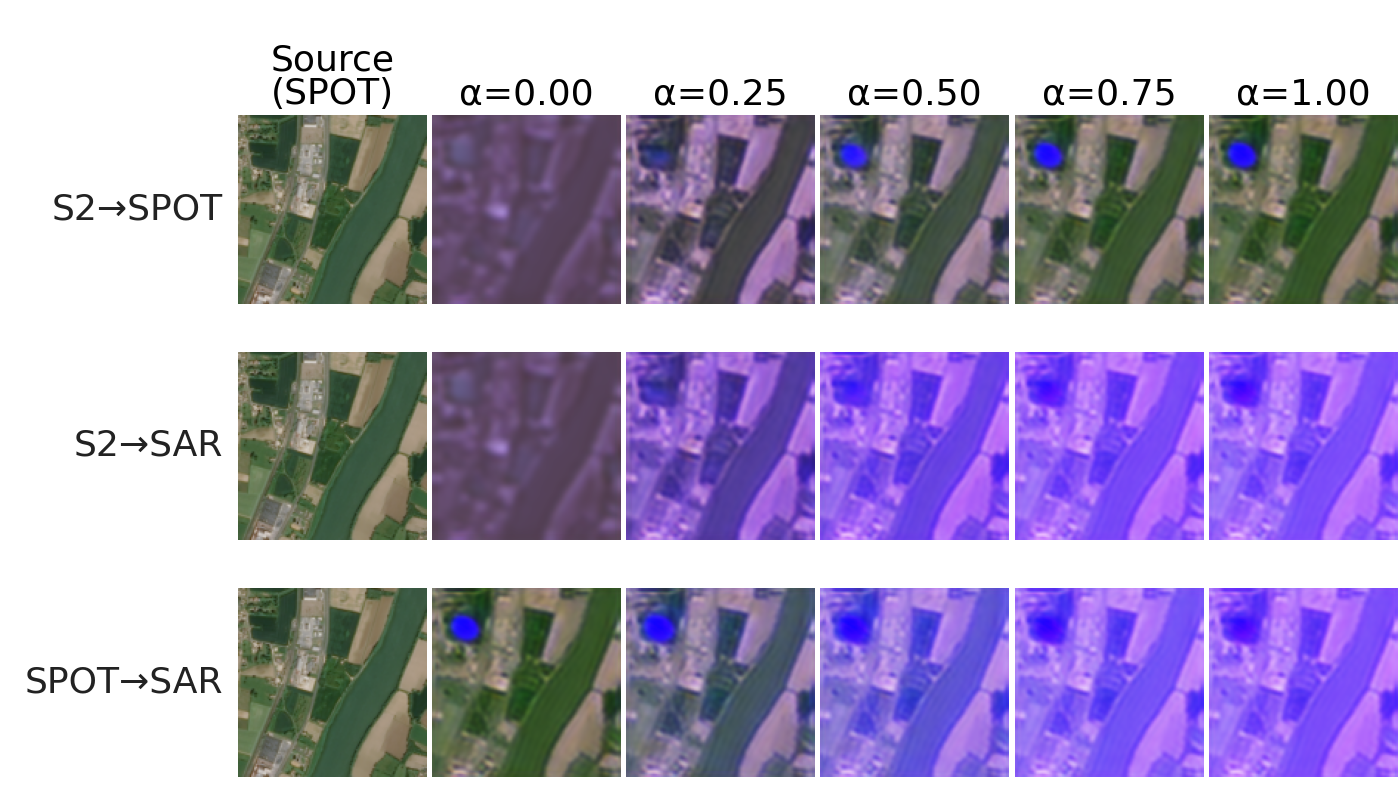
\includegraphics[width=\columnwidth]{figures/fig_interp_compact.png}
\caption{Interpolation of the style vector between two domain centroids, $z(\alpha)=(1-\alpha)\bar z_a+\alpha\bar z_b$ renormalized to unit length, applied to one held-out SPOT~6/7 source patch (first column). Each row is a pair of domains $a \rightarrow b$ and $\alpha$ runs from the style of $a$ ($\alpha=0$) to the style of $b$ ($\alpha=1$). The patch was chosen by a fixed random seed before inspection.}
\label{fig:interp}
\end{figure}

The architectural objectives of Table~\ref{tab:gap} are achieved: there is no labeling of the domain, a single generator for all the ordered pairs of three domains, and a continuous 64-dimensional domain code. None of the cited methods were trained on the same data as used for this work, and the numbers published for these methods are from other data and tasks, so any comparison to the quality of the result is not warranted, and no claim is made that the approach is better than SS(DA)$^2$, StarGAN~v2, or any of the other methods.

\section{Limitations}
\label{sec:limitations}
The above results have some restrictions. First, the held-out patches are from one Sentinel-2 tile, and the training set is largely from two other tiles, and so the results are a blend of model quality and a shift towards a different region; domain centroids are from different regions to the patches they're applied to. Second, there is no simultaneous modality, limiting the ability to agree at the pixel level with the co-registered reference, and there are artifacts in the preprocessing (saturated SAR channel and synthetic fourth SPOT channel). Third, for each model, the training was performed only once on a CPU with only 12 epochs of the generator and 10 epochs of the encoder (Sec.~\ref{sec:setup}), and the training loops were not seeded, no run-to-run variation was tested, no ablation of the six generator losses was performed, and no other method of translation was trained on the same data. Fourth, PSNR and SSIM are used for the degree of agreement with a co-registered image, not for realism, and the rate of style transfer is evaluated by the same encoder used for conditioning the generator. Fifth, only three sensor domains, one geographic setting and 1,500 of 2,433 locations were utilized; the larger MSC-France corpus that was foreseen forencoder pretraining and the angle-conditioning were not used. Finally, generalisation of unseen sensor pairs and downstream accuracy are not assessed.

\section{Conclusion and Future Work}
The proposed framework was a novel multi-domain self-supervised adaptation framework for satellite-based image data, which consisted of two main components: a contrastive domain encoder for learning label-free, continuous embeddings of the sensor style of the images, and an AdaIN-conditioned generator for generating an image in an arbitrary target style, given a source patch and its learned embedding from the domain encoder. The framework has the potential to comply with the design goals at the architectural level: No domain labels, one model for all ordered domain pairs, a continuous domain code, trained on real PASTIS-HD imagery (Sentinel-2, SPOT~6/7, Sentinel-1 SAR). There is a limited measured quality: the encoder identifies the sensor moderately (65.8\% vs 33.3\% chance) and the generator preserves the structure of the scene and uses the style vector, but cannot reproduce the radiometry of the measured sensor; translations into Sentinel-2 do not work.

Future work will involve (i) replacing the augmented-view positives with sensor-aware positive pairs based on spatial and temporal proximity and pretraining on a larger corpus MSC-France; (ii) fixing data issues found here, including all PASTIS-HD patches, a tile-stratified split and temporally matched acquisitions, a non-saturating SAR channel; (iii) training wider networks longer on a GPU with seeded runs, loss ablations and same-data baselines; and (iv) testing leave-one-domain-pair-out and zero-shot (SpaceNet~6) generalization and downstream crop classification and segmentation.

\bibliographystyle{IEEEtran}
\bibliography{references}

\end{document}
